% Discussion slides are outside the timed core. Their source labels name the dissertation.
\begin{frame}{Discussion guide}
\fontsize{8}{9.5}\selectfont
{\scriptsize\textbf{Further detail:} \ifdefined\DefenseNotes time-surface regression and contrast maximization; the full stereo arc (Chapter 4); references\else\hyperlink{flowdetails}{time-surface regression and contrast maximization}; \hyperlink{stereoarc}{the full stereo arc (Chapter 4)}; \hyperlink{references}{references}\fi.}\par\vspace{-1mm}
\begin{columns}[T]
\column{.48\textwidth}
\textbf{Observation and temporal inversion}
\begin{itemize}
\item Minimal uniqueness condition / reference level
\item Measure-valued continuous-time limit
\item Signal gain versus noise gain
\item \ifdefined\DefenseNotes Metrics; real time; solve; core rate; problem size\else\hyperlink{metricguide}{Metrics}; \hyperlink{realtime}{real time}; \hyperlink{tridiagcost}{solve}; \hyperlink{corerate}{core rate}; \hyperlink{temporalcost}{problem size}\fi
\item Kernels; \ifdefined\DefenseNotes $\Lam(\mathbf y)$ stability\else\hyperlink{adaptivelipschitz}{$\Lam(\mathbf y)$ stability}\fi
\item \ifdefined\DefenseNotes Grayscale scenes; MVSEC events in space-time and summed\else\hyperlink{scenesgray}{Grayscale scenes}; MVSEC events \hyperlink{mvsecevents3d}{in space-time} and \hyperlink{mvsecaccum}{summed}\fi
\end{itemize}
\textbf{Flow analysis}
\begin{itemize}
\item Weak Euler equation and boundary condition
\item Full proof, stability, and discrete sweeps
\item Exact block-Jacobi spectral argument
\item Anisotropy; \ifdefined\DefenseNotes $\lambda,\alpha\to0$; event-free regions\else\hyperlink{weakreg}{$\lambda,\alpha\to0$}; \hyperlink{harmonicfill}{event-free regions}\fi
\item Regression, projection, \ifdefined\DefenseNotes evaluation; splines\else\hyperlink{flowprotocol}{evaluation}; \hyperlink{splinecoercive}{splines}\fi
\item \ifdefined\DefenseNotes Straight-edge aperture model\else\hyperlink{aperturemodel}{Straight-edge aperture model}\fi
\end{itemize}
\column{.48\textwidth}
\textbf{Stereo analysis}
\begin{itemize}
\item Chapter 4 results summary
\item Mean-zero conditioning
\item Cost ellipsoid and observation perturbations
\item IRLS contraction proof
\item Fixed points versus likelihood stationarity
\item Implemented scoring and aggregation
\end{itemize}
\textbf{Evidence and interpretation}
\begin{itemize}
\item Depth coverage; \ifdefined\DefenseNotes alignment; sensitivity\else\hyperlink{stereoalignment}{alignment}; \hyperlink{depthsensitivity}{sensitivity}\fi
\item \ifdefined\DefenseNotes One lemma behind the uniqueness results\else\hyperlink{complementarity}{One lemma behind the uniqueness results}\fi
\item Contribution; \ifdefined\DefenseNotes parameters; learning\else\hyperlink{paramchoice}{parameters}; \hyperlink{learnedfit}{learning}\fi
\item Literature anchors and source map
\end{itemize}
\end{columns}
\talknote{Use as an appendix index.}{The following slides answer questions. PDF section bookmarks and the source-map file make it possible to find their manuscript origins.}{Each discussion slide has notes that give the proof mechanism or a suggested concise answer.}
\end{frame}



\begin{frame}{One penalty entry makes the temporal solve unique}
For arbitrary $\Lam$, the exact algebraic criterion is
\[\A^\top\A+\Lam^\top\Lam\succ0
\quad\Longleftrightarrow\quad\ker\A\cap\ker\Lam=\{0\}.\]
\vspace{2mm}
On a connected chain, $\ker\A=\operatorname{span}\{\mathbf1\}$, so one nonzero penalty entry, a fixed reference value, or a zero-mean constraint each makes the solve unique.
% source detail: Ch. 2, lem:nullspace; Ch. 4, discussion following lem:A\_spectrum.
\src{\dref{Lemma}{lem:nullspace}; discussion following \dref{Lemma}{lem:A_spectrum}.}
\talknote{Question: why use a full positive diagonal?}{The main theorem's positive diagonal is a strong sufficient hypothesis with an immediate quantitative lower bound. Weaker conditions also give definiteness. The kernel-intersection argument shows the minimal condition. A one-point anchoring penalty gives definiteness, but its eigenvalue bound differs from lambda\_min squared when other diagonal entries are zero.}{An explicit zero-mean parameterization can avoid penalizing the unobserved offset. It changes the estimator: the original magnitude penalty also attenuates nonconstant modes and controls noise. A chosen reference level fixes the estimate's offset; the absolute brightness baseline needs a measurement. Why: the quadratic form vanishes exactly when $\A\mathbf z=0$ and $\Lam\mathbf z=0$. Any reference level resolves the mathematical ambiguity; a measured reference adds physical information.}
\end{frame}

\begin{frame}{The event measure has a jump primitive}
At one pixel, set $\mu=\sum_jp_j\delta_{s_j}$, and choose a consistent right-continuous primitive
\[g(t)=f_0+\mu((t_0,t]),\qquad g(b)-g(a)=\mu((a,b]).\]
For a standard smooth compactly supported unit-mass kernel,
\[e_h=\mu*\phi_h,\qquad g_h(t)=f_0+\int_{t_0}^t e_h(\xi)\,d\xi.\]
For finitely many interior events, $g_h\to g$ in $L^1$ as $h\downarrow0$.
% source detail: Ch. 2, subsubsec:ode; endpoint convention made explicit here.
\src{Continuous-time formulation (\drefpage{subsubsec:ode}); endpoint convention made explicit here.}
\talknote{Question: what is the continuous-time problem?}{A finite atomic measure has a bounded-variation cumulative primitive. For a nonzero interior atom its derivative is singular, so it cannot have an L2 weak derivative and is not H1. With finite standard bounded kernels of positive width, the smoothed driver is L2 and its primitive is H1. Arbitrary L1 alone would only guarantee W1,1.}{The bin convention (a,b] here matches the right-continuous process exactly. Alternative half-open bins are valid with a compatible representative or an explicit no-boundary-events assumption. The difference quotient is the integrated event increment divided by the time step; the discrete A in the presentation computes increments. $g$ is a $BV$ function with a jump at each event, so it lies outside $H^1$; it is the unregularized cumulative-event surrogate. The model uses increments, $\A\mathbf f\approx\mathbf y$, with consistent interval conventions.}
\end{frame}

\begin{frame}{The penalty attenuates low modes and bounds the noise gain}
For the unweighted monocular model with scalar $\lambda>0$,
\[\mathbf f^*=(\A^\top\A+\lambda^2\mathbf I)^{-1}\A^\top\mathbf y.\]
\renewcommand{\arraystretch}{1.45}
\begin{tabular}{ll}\toprule Input & Output modal gain\\\midrule
Latent signal & $g_k/(g_k+\lambda^2)$\\
Difference observation & $\sqrt{g_k}/(g_k+\lambda^2)$\\
White difference noise & $\sigma^2g_k/(g_k+\lambda^2)^2$\\\bottomrule
\end{tabular}
\vspace{3mm}
% source: Ch. 4 prop:noise_gain; max_{g>=0} g/(g+lambda^2)^2=1/(4lambda^2), derivative vanishes at g=lambda^2.
\[\max_{g\ge0}\frac{g}{(g+\lambda^2)^2}=\frac1{4\lambda^2}.\]
% source detail: Ch. 4, thm:frequency\_response, prop:noise\_gain.
\src{\dref{Theorem}{thm:frequency_response}, \dref{Proposition}{prop:noise_gain}.}
\talknote{Question: what kind of filter is this?}{Take the singular-value decomposition A=U Sigma V\textasciicircum{}T. The reconstruction operator maps left singular modes of y to right singular modes with amplitude sqrt(g)/(g+lambda squared). Multiplying by A for noiseless y=A f\_true yields the latent-signal gain g/(g+lambda squared). For white independent observation noise the output covariance diagonalizes in the same right modes and its modal variance is sigma squared times the squared observation gain.}{Differentiate g/(g+a)\textasciicircum{}2 with a=lambda squared: the derivative has sign a-g, so the continuous maximum is 1/(4a) at g=a. The discrete finite-chain maximum may be smaller because its available eigenvalues need not contain a. These formulas are for a scalar penalty and equal weights. Rows: the latent-signal gain attenuates low modes most; the observation row is the noise amplitude transfer; the last row is the reconstructed modal variance.}
\end{frame}

\begin{frame}{Kernel rankings change with the scene}
\small\renewcommand{\arraystretch}{1.2}
\begin{center}\begin{tabular}{lrrrr}\toprule
&\multicolumn{2}{c}{MVSEC indoor}&\multicolumn{2}{c}{MVSEC outdoor}\\
Kernel&PSNR&CN&PSNR&CN\\\midrule
% source: Ch. 2 tab:bump_avg_indoor and tab:bump_avg_outdoor, B-spline rows. CN: mean per-pixel condition number (Ch. 2 tables; /scratch/dblauvel/ch2_recompute_20261103_p60/results_actual_cn/table_cn.tsv).
B-spline&8.66&259.87&7.29&258.68\\
% source: Ch. 2 tab:bump_avg_indoor and tab:bump_avg_outdoor, Delta rows.
Delta&8.49&261.98&7.28&267.99\\
% source: Ch. 2 tab:bump_avg_indoor and tab:bump_avg_outdoor, Gaussian rows.
Gaussian&8.68&259.79&7.23&259.42\\
% source: Ch. 2 tab:bump_avg_indoor and tab:bump_avg_outdoor, Rectangular rows.
Rectangular&8.58&261.10&7.31&263.33\\\bottomrule
\end{tabular}\end{center}
% source detail: Ch. 2, tab:bump\_avg\_indoor, tab:bump\_avg\_outdoor.
\src{\dref{Table}{tab:bump_avg_indoor}, \dref{Table}{tab:bump_avg_outdoor}.}
\talknote{Question: why does a smoothing kernel change conditioning?}{The matrix K=A\textasciicircum{}T A+Lambda\textasciicircum{}T Lambda contains the bump kernel only through the observations and the weights derived from them. However Lambda is computed adaptively from represented observations. Changing aggregation can change those weights, hence the numerical matrix. With the same sigmoid weights, the four kernels give mean per-pixel condition numbers of 259 to 268, while the choice of weight rule moves it from 2.4 to 265.}{The table reports the mean per-pixel condition number. PSNR differs by at most 0.2 dB across kernels, and its ordering differs indoors and outdoors. The positivity theorem gives a sufficient worst-case bound, independent of the empirical ranking. The temporal operator stays the same across kernels; the represented data and adaptive penalties change. Conditioning and reconstruction bias are separate properties, and reference-image scores also measure the baseline the model selects.}
\end{frame}

\begin{frame}[t,label=metricguide]{Each reconstruction score measures one property}
\footnotesize
\renewcommand{\arraystretch}{1.15}
\begin{tabular}{p{.17\textwidth}p{.35\textwidth}p{.37\textwidth}}
\toprule Quantity & What it compares & What it establishes\\\midrule
PSNR / SSIM & Reconstruction and reference images & Image agreement under the scoring convention\\
TC / TG & Temporal changes in the output & Smoothness of the returned sequence\\
ERC & Magnitudes of reconstructed changes and represented events & Correlation with event activity\\
CN & Sensitivity of each pixel's system matrix, averaged over pixels & A numerical conditioning diagnostic\\\bottomrule
\end{tabular}
\src{Evaluation metrics (\drefpage{subsubsec:metrics}); \dref{Table}{tab:metrics_summary}; SSIM~\cite{wang2004ssim}.}
\talknote{Question: how is each metric computed, and what does it establish? About 2 minutes if all definitions are requested.}{PSNR converts the peak-squared to mean-squared pixel-error ratio to decibels. SSIM combines local means, variances and covariance to compare luminance, contrast and structure. EPI correlates mean-image gradient magnitudes with the normalized event-count map. ERC correlates absolute frame changes with absolute bump-integrated event data. TC exponentiates the negative RMS frame change divided by the reconstruction range. TG averages absolute frame changes. TV averages the sum of absolute horizontal and vertical gradients. SC averages each frame's fraction of Fourier power in the central low-frequency disk. CN divides the largest singular value of each active pixel's matrix by its smallest, averaged over the active pixels.}{Use the script for aggregation and degenerate-case details. A constant sequence has maximal TC and zero ERC under the conventions, separating smoothness from event consistency. CN describes the specified diagnostic matrix. Answer only the definitions requested; the existing slide remains an interpretation guide. % source: Ch. 2 metric definitions and degenerate-case conventions, lines 603-611.
A check on interpretation: a constant sequence has $\mathrm{TC}=1$ and $\mathrm{ERC}=0$, so smoothness alone rewards a static output.}
\end{frame}

\begin{frame}[t,label=realtime]{One core streams DAVIS data at 0.39 of real time}
\footnotesize
\textbf{CPU measurements} (one HPC CPU node; float32; processing time $\div$ recording time)\par\smallskip
% source: /scratch/dblauvel/thesis_rerun_20261024/edge/run_2945746/{window,stream}/bench_{davis_pendulum,hs_gun_bullet_mug}_amd041.orc.gmu.edu_*.json (Slurm 2945746, revision cdca5a4, empty source.diff; AMD node amd041; batch: active-pixel solve, median of 10 windows; streaming: 500 intervals of 2 ms).
\begin{tabular}{llrrrrr}\toprule
& & & \multicolumn{2}{c}{Batch: 100\,ms, $N=50$} & \multicolumn{2}{c}{Streaming: 2\,ms steps}\\
Data & Pixels & Events/s & 1 thr. & 8 thr. & 1 thr. & 8 thr.\\\midrule
DAVIS346 pendulum & 90k & 0.25\,M & 0.04 & 0.008 & 0.39 & 0.06\\
Cup & 307k & 2.3\,M & 1.0 & 0.19 & 1.3 & 0.21\\\bottomrule
\end{tabular}\par\bigskip
% source: run_2945746 window; state: tridiag.py StreamingReconstructor, 4 float32 arrays per pixel (1.4 MB DAVIS, 4.9 MB cup).
{\small Values below 1 run faster than the recording. State: 16 bytes per pixel.\par}
\vfill{\fontsize{6.5}{8}\selectfont\color{muted}Source: edge implementation, October 2026 CPU timings and MATLAB comparison.\par}
\talknote{Question: can the reconstruction run in real time? About 60 seconds.}{These are measurements of the Chapter 2 estimator on one CPU node. DAVIS data take about four percent of real time on one thread for batch windows. The 640 by 480 cup recording at 2.3 million events per second runs at real time on one thread for batch windows and 1.3 for streaming; eight threads bring both to about a fifth of real time. Streaming state is four float32 numbers per pixel: 1.4 MB for DAVIS346 and 4.9 MB for the cup. Batch processes a complete window; streaming returns the newest endpoint of a growing prefix with finalized interval observations.}{The terminal weight repeats the last interval weight, so its diagonal is one plus that weight squared. Streaming matches the full mathematical batch solve on each growing prefix; the batch code skips pixels whose net event sum is zero, so compare the two on the same pixel set. Earlier output frames can change when later data arrive. A sliding window changes the left boundary and needs additional handling. Backup 79 covers complexity, memory, and low-power choices. % source: repo_outputs/audits/thesis_rerun_20261024/validation/run_2940318/full.log; run_2945746 window, DAVIS 1 thread rtf_all 0.434 vs rtf_active 0.041.
Speed: $O(N)$ tridiagonal solves on event-active pixels (tenfold fewer on DAVIS). MVSEC: 0.03\,s tridiagonal vs 1.5\,s dense, matching MATLAB within $10^{-15}$.}
\end{frame}

\begin{frame}{The weak equation supplies the natural boundary condition}
For every $\boldsymbol\eta\in H^1(\Omega;\R^2)$,
\[\int_\Omega(\B\vct^*-b)\cdot\boldsymbol\eta
+\alpha^2\int_\Omega\nabla\vct^*:\nabla\boldsymbol\eta=0.\]
Interior tests give the distributional equation
\[-\alpha^2\Delta\vct^*+\B\vct^*=b.\]
Since the coefficients imply $\Delta\vct^*\in L^2$, Green's identity gives
\[\partial_n\vct^*=0\quad\text{in }H^{-1/2}(\partial\Omega;\R^2).\]
% source detail: Ch. 3, time-surface, voxel and structure-tensor Euler--Lagrange theorems.
\src{\dref{Theorem}{thm:euler_lagrange}, \dref{Theorem}{thm:euler_lagrange_vox_projection}, and \dref{Theorem}{thm:euler_lagrange_tensor}.}
\talknote{Question: which boundary condition is imposed?}{The energy is minimized over the full space H1, so natural Neumann conditions emerge from the first variation. Compactly supported smooth tests first give the interior equation. B v and b are in L2, hence the distributional Laplacian is L2, so the gradient has a weak normal trace.}{Returning to arbitrary H1 tests, generalized Green's identity leaves a boundary pairing with their traces. Surjectivity of the trace map makes the normal trace zero. The anisotropic form replaces grad by D grad and yields a conormal condition n\textasciicircum{}T D grad v=0. No differentiability of D is needed for its weak formulation. The theorem works with $H^1$ fields and weak traces on a Lipschitz domain.}
\end{frame}

\begin{frame}{Proof: control the mean and the fluctuation separately}
Decompose $\vct=\underbrace{\bar{\vct}}_{\text{common drift (pan)}}+\underbrace{\mathbf w}_{\text{variation across the image}}$, with $\int_\Omega\mathbf w=0$.
\[\norm{\mathbf w}_{L^2}\le C_P\norm{\nabla\vct}_{L^2}.\]
Let $\beta_B=\norm{\B}_{L^\infty}$ and $m=\min_{|\mathbf e|=1}\mathbf e^\top(\int_\Omega\B)\mathbf e>0$ (how well the edges cover every direction).
% source: Ch. 3 proof of thm:unified_wellposedness, eq:mean_control.
\[m|\bar{\vct}|^2\le2\int_\Omega\vct^\top\B\vct+2\beta_BC_P^2\norm{\nabla\vct}_{L^2}^2.\]
Therefore the bilinear form satisfies
% source: Ch. 3 proof of thm:unified_wellposedness; admissible lower bound, not optimal.
\[\mathcal B(\vct,\vct)=\int\vct^\top\B\vct+\alpha^2\int|\nabla\vct|^2
\ge c_0\norm{\vct}_{H^1}^2,\qquad
c_0=c_0(\Omega,\alpha,\beta_B,m).\]
% source detail: Ch. 3, proof of thm:unified\_wellposedness.
\src{proof of \dref{Theorem}{thm:unified_wellposedness}; Lax--Milgram~\cite{lax1954parabolic}.}
\talknote{Question: how exactly does the proof control the mean? About 2 minutes.}{The gradient seminorm misses exactly the constant vector fields. Write the field as its mean plus a zero-mean part. Poincar\'e controls the latter. Use $\norm{\B^{1/2}\bar{\vct}}_{L^2}\le\norm{\B^{1/2}\vct}_{L^2}+\norm{\B^{1/2}\mathbf w}_{L^2}$, square with the factor-two inequality, and bound the fluctuation term by $\beta_BC_P^2\norm{\nabla\vct}_{L^2}^2$. Positive definiteness of the integrated matrix controls the mean.}{An admissible lower bound is $c_0=\min\{m/(2|\Omega|),\alpha^2/(1+C_P^2+2|\Omega|\beta_BC_P^2/m)\}$. Insert it into $\norm{\vct}_{H^1}^2=|\Omega||\bar{\vct}|^2+\norm{\mathbf w}_{L^2}^2+\norm{\nabla\vct}_{L^2}^2$. Lax--Milgram gives the unique minimizer. For fixed positive $\beta_B,\alpha$, this lower bound deteriorates linearly as $m$ decreases. Scene terms: mean = common drift (camera pan), fluctuation = variation across the image; smoothness charges nothing for a pan, so the edges must fix it.}
\end{frame}

\begin{frame}{The flow is Lipschitz in its coefficients}
\small
Suppose two coefficient pairs share bounds
\[\norm{\B_i}_{L^\infty}\le \beta_B,\qquad\lambda_{\min}\!\left(\int\B_i\right)\ge m>0,
\qquad\norm{b_i}_{L^2}\le R_b.\]
Here $c_0=c_0(\Omega,\alpha,\beta_B,m)$ is independent of $b_i$.
For $\mathbf z=\vct_1^*-\vct_2^*$,
\[\mathcal B_1(\mathbf z,\mathbf z)
=\int(b_1-b_2)\cdot\mathbf z+\int\mathbf z^\top(\B_2-\B_1)\vct_2^*,\quad\text{hence}\]
\vspace{-2mm}
\[\norm{\mathbf z}_{H^1}\le c_0^{-1}\norm{b_1-b_2}_{L^2}
+c_0^{-2}R_b\norm{\B_1-\B_2}_{L^\infty}.\]
% source detail: Ch. 3, thm:unified\_wellposedness, eq:abstract\_stability.
\src{\dref{Theorem}{thm:unified_wellposedness}, \dref{Eq.}{eq:abstract_stability}.}
\talknote{Question: how is the stability bound derived? About 75 seconds.}{The same coercivity constant works on both coefficient pairs because the quantitative bounds are shared. Subtract their weak equations and test with the solution difference. Cauchy--Schwarz controls the right side, and $\norm{\vct_2^*}_{H^1}\le R_b/c_0$ follows from its own weak equation. Divide by $\norm{\mathbf z}_{H^1}$ if it is nonzero.}{The conclusion is stability of the chosen estimator. The estimate may become poor as $m\to0$. If a density-dependent diffusion tensor is recomputed, the regularizer also changes; its $L^\infty$ perturbation must enter the bound. Scene terms: coefficient changes come from timestamp jitter, binning, and noise events; small $m$ is the stripe case in the talk. % source: Ch. 3, paragraph after the proof of thm:unified_wellposedness.
Scene terms: jitter, binning, and noise events change the coefficients, and the constants grow as $m$ shrinks, as in the stripe scene. Accuracy: the bound concerns the minimizer of the chosen energy; its distance from the true motion depends on coefficient accuracy and on $H^1$ smoothing across motion boundaries (known-motion AEE, page 85).}
\end{frame}

\begin{frame}{Jacobi sweeps converge to the unique discrete flow}
\small
Fix $\alpha>0$, $q_i>0$, and $\B_i=\B_i^\top\succeq0$ on a connected graph with
$w_{ij}=w_{ji}\ge0$ and degree $d_i=\sum_jw_{ij}>0$.
\begin{block}{One simultaneous block-Jacobi sweep}
% source: Ch. 3 thm:convergence and cor:convergence_psd_blocks; normal-equation block update with positive q_i absorbed into B_i and b_i.
\[
\underbrace{(q_i\B_i+\alpha^2d_i\mathbf I_2)}_{\text{local }2\times2\text{ matrix}}
\vct_i^{(k+1)}
=q_i b_i+\alpha^2\sum_jw_{ij}\vct_j^{(k)}.
\]
\end{block}
% source: Ch. 3 thm:convergence and cor:convergence_psd_blocks, extended to q_i>0 by absorbing q_i into B_i.
If $\sum_iq_i\B_i\succ0$, the discrete energy has a unique minimizer, and these sweeps converge to it from every initial field.
% source detail: Ch. 3, cor:vox\_projection\_wellposed; positive-$q_i$ extension of thm:convergence and cor:convergence\_psd\_blocks.
\src{\dref{Theorem}{thm:convergence} and \dref{Corollary}{cor:convergence_psd_blocks}; extension to positive node factors $q_i$.}
\talknote{Question: how is the flow computed? About 90 seconds.}{Each node stores a two-component velocity. With coefficients fixed, the normal equation at node i has the local data matrix $q_i\B_i$ plus alpha squared times the weighted degree. Move the neighboring velocities to the right, and use their values from the previous sweep. This gives the displayed two-by-two solve. The $q_i b_i$ term carries the local observations, and the weighted neighbor sum carries the previous surrounding field. Compute every new velocity from the same old field, then replace the whole field and repeat.}{The theorem assumes a connected graph, symmetric nonnegative edge weights, positive degrees and node factors, PSD data blocks, and a positive-definite sampled Gram matrix. For this graph operator, zero graph energy forces a constant field, and the sampled data remove that constant null direction. Write $H=D-R$, where $D$ contains the local two-by-two blocks and $R$ contains the neighbor couplings. Both $D-R$ and $D+R$ are positive definite: possible alternating constants of the signless graph form are removed by the same sampled data condition. Hence the spectrum of the similar symmetric Jacobi matrix lies in $(-1,1)$. This proves convergence of the simultaneous schedule from every initial field. Match a representation's stencil and update schedule to these hypotheses before applying the result. Scene terms: information spreads one neighbor per sweep.}
\end{frame}

\begin{frame}{The Jacobi iteration matrix has spectral radius below one}
Absorb $q_i$ into $\widehat\B_i=q_i\B_i\succeq0$. Set
\[D_i=\alpha^2d_i\mathbf I+\widehat\B_i,\qquad R_{ij}=\alpha^2w_{ij}\mathbf I.\]
For symmetric nonnegative edge weights,
\[\mathbf z^\top(D\mp R)\mathbf z=\sum_i\mathbf z_i^\top\widehat\B_i\mathbf z_i
+\alpha^2\sum_{\{i,j\}}w_{ij}\norm{\mathbf z_i\mp\mathbf z_j}^2.\]
Connectedness and $\sum_i\widehat\B_i\succ0$ eliminate both constant and alternating constant zero modes (the latter on bipartite graphs).
\[D-R\succ0,\quad D+R\succ0\quad\Rightarrow\quad
-\mathbf I\prec D^{-1/2}RD^{-1/2}\prec\mathbf I.\]
% source detail: Ch. 3, extension of thm:convergence and cor:convergence\_psd\_blocks by absorbing $q_i$ into $\widehat\B_i$. $\alpha>0$, $d_i>0$.
\src{extension of \dref{Theorem}{thm:convergence} and \dref{Corollary}{cor:convergence_psd_blocks} by absorbing $q_i$ into $\widehat\B_i$. $\alpha>0$, $d_i>0$.}
\talknote{Question: why does SPD suffice here for Jacobi?}{The special graph form proves more than SPD alone. For D-R, a zero edge sum forces equality of neighbors, so all node vectors equal a constant. For D+R, it forces opposite vectors on every edge; on a bipartite graph they are alternating copies of one constant vector, while an odd cycle forces zero. The sampled PSD data blocks eliminate any nonzero constant or alternating constant.}{D is SPD because alpha and each degree are positive. Conjugate D plus or minus R by D\textasciicircum{}{-1/2}; the two positivity statements bound the symmetric spectrum between minus and plus one. D\textasciicircum{}{-1}R is similar to it, hence its spectral radius is below one and repeated simultaneous sweeps converge. Conclusion: the Jacobi iteration matrix is similar to a symmetric matrix with spectral radius strictly below one.}
\end{frame}

\begin{frame}{Nagel--Enkelmann smoothing stays uniformly elliptic}
For the normalized Nagel--Enkelmann tensor~\cite{nagel1986investigation}, write $g=\nabla\rho_{\rm evt}$ and $\gamma_{\rm NE}>0$:
% source: Ch. 3 eq:ne_tensor; this is the normalized variant used in the dissertation.
\[\mathbf D=\frac{g^\perp(g^\perp)^\top+\gamma_{\rm NE}^2\mathbf I}{|g|^2+\gamma_{\rm NE}^2}.
\]
Its tangent and normal eigenvalues are
\[1,\qquad\frac{\gamma_{\rm NE}^2}{|g|^2+\gamma_{\rm NE}^2}.\]
If $g\in L^\infty$,
\[\theta\mathbf I\preceq\mathbf D\preceq\mathbf I,\qquad
\theta=\frac{\gamma_{\rm NE}^2}{\norm{g}_{L^\infty}^2+\gamma_{\rm NE}^2}>0.\]
% source detail: Ch. 3, normalized variant of eq:ne\_tensor, lem:ne\_elliptic, cor:structure\_wellposedness.
\src{normalized variant of \dref{Eq.}{eq:ne_tensor}, \dref{Lemma}{lem:ne_elliptic}, \dref{Corollary}{cor:structure_wellposedness}.}
\talknote{Question: can an adaptive diffusion tensor retain well-posedness?}{For a fixed, bounded, symmetric tensor with a common strictly positive lower eigenvalue bound, the Poincare/coercivity argument survives. Merely saying positive definite at each point is insufficient if eigenvalues approach zero. The normalized Nagel--Enkelmann form provides an explicit uniform floor when the density gradient is bounded.}{The tensor reduces penalties on normal-direction flow variations and preserves the tangent-direction penalty. If it is recomputed after data perturbation, stability includes ||D\_1-D\_2||\_infty. Event-density edges need not coincide with motion boundaries. The CM tensor alpha\_ani squared J plus epsilon I has the opposite directional effect: it increases the normal-direction penalty. So the tensor reduces diffusion across event-density edges, and coercivity holds with constant $\alpha^2\theta$.}
\end{frame}

\begin{frame}{A variable diffusion tensor must stay inside the divergence}
For differentiable $\mathbf D$,
\begin{align*}
\nabla\!\cdot(\mathbf D\nabla u)
&=D_{11}u_{xx}+2D_{12}u_{xy}+D_{22}u_{yy}\\
&\quad+(\partial_xD_{11}+\partial_yD_{12})u_x
+(\partial_xD_{12}+\partial_yD_{22})u_y.
\end{align*}
% source: Ch. 3 eq:aniso_divergence_expansion and subsequent counterexample.
Take $\rho_{\rm evt}=x^2/2$, $\gamma_{\rm NE}=1$, and $u=x$:
\[\mathbf D=\operatorname{diag}\!\left(\frac1{1+x^2},1\right),\qquad
\nabla\!\cdot(\mathbf D\nabla u)=\frac{-2x}{(1+x^2)^2}\not\equiv0.\]
All second derivatives of $u$ vanish, so the whole value comes from the first-order terms.
% source detail: Ch. 3, rem:aniso\_discretization.
\src{Anisotropic numerical discretization (\drefpage{rem:aniso_discretization}).}
\talknote{Question: can you just replace the Laplacian by a tensor-weighted Hessian?}{Only for a constant tensor or when its coefficient-derivative contributions vanish. With a variable tensor the product rule supplies first-order terms. The affine test field exposes their importance particularly clearly, because its Hessian vanishes identically while its divergence-form diffusion does not.}{For merely L-infinity D, those classical coefficient derivatives may not exist. Keep the weak form integral grad eta transpose D grad u; it requires no derivative of D. A flux-consistent discretization should approximate that divergence form directly.}
\end{frame}

\begin{frame}{Curvature bias and noise set the regression radius}
For full disks on a square lattice of spacing $h$, with $r/h$ large,
% source: Ch. 3 prop:ts_regression_bound(iv), eq:ts_radius_surrogate.
\[Q\sim\frac{\pi r^4}{4h^2}\mathbf I,\qquad
U_h(r)=\frac4{81}L_H^2r^4+\frac8\pi\sigma^2h^2r^{-4}.\]
The minimum of this leading expression, when all parameters are positive, is
% source: Ch. 3 radius-selection paragraph; r*^8=(162/pi) sigma^2 h^2 / L_H^2.
\[r^*=(162/\pi)^{1/8}(\sigma h/L_H)^{1/4}.\]
% source detail: Ch. 3, prop:ts\_regression\_bound and Radius selection as a heuristic.
\src{\dref{Proposition}{prop:ts_regression_bound} and Radius selection as a heuristic.}
\talknote{Question: is your radius choice optimal?}{Differentiate the positive leading bias-squared plus variance expression, which scales as A r\textasciicircum{}4 + B r\textasciicircum{}{-4}. Its stationary radius obeys r\textasciicircum{}8=B/A. The resulting scaling is a guide to how timestamp noise, lattice spacing, and curvature interact.}{The exact finite-design bound uses lattice sums. The asymptotic error can have either sign, so the leading surrogate approximates the bound from either side. The formula also requires positive curvature Lipschitz bound and noise, a large radius in lattice units, and inclusion in the smoothness neighborhood. Boundary truncation or sparse event support can destroy central symmetry and alter the bias. Scope: the full disk lies in a region with the asserted smoothness bound, and $U_h$ is the asymptotic form of the finite-design bound, so $r^*$ is a heuristic. For an affine time surface the curvature bias is zero and the variance term alone sets the radius, favoring larger disks.}
\end{frame}

\begin{frame}{Uniform and OLS weights first differ on cubics}
The continuous OLS temporal slope over $[s,s+T]$ is
\[\widehat\beta=\int_s^{s+T}w_s(t)V_t(t)\,dt,\qquad
w_s(t)=\frac{6(t-s)(s+T-t)}{T^3}.\]
Its transport-consistent spatial partner is the same $w_s$-weighted projection.
Pairing it with a uniform projection gives residual
\[\vct\cdot\nabla\int_s^{s+T}(T^{-1}-w_s(t))V(\mathbf x,t)\,dt.\]
% source: Ch. 3 derivative-operator qualifications, transported cubic counterexample.
For $V(x,t)=(2+x-t)^3$, $\vct=(1,0)$, $s=0$, $T=1$, this residual is $1/10$.
% source detail: Ch. 3, subsec:vox\_projection, consistent derivative-operator discussion.
\src{\dref{Section}{subsec:vox_projection}, consistent derivative-operator discussion.}
\talknote{Question: why distinguish the implementation from exact transport?}{Integration by parts in the OLS slope formula yields the parabolic weight w\_s on the temporal derivative. Integrating the transport equation with that weight gives a correspondingly weighted spatial gradient. Using a uniform mean on one side and an OLS slope on the other generally gives a residual mismatch.}{Uniform and OLS weights share zeroth and first temporal moments, so transported polynomials through degree two have zero mismatch. The cubic example supplies an actual derivative mismatch. This is a representation-coefficient error that the abstract stability theorem can address if its norm and identifiability hypotheses are controlled. Derivative consistency is a separate check from well-posedness of a fixed-coefficient energy.}
\end{frame}

\begin{frame}{Mean-zero profiles keep the stereo system definite}
In the unweighted scalar model, restrict to
\[\mathcal V_0=\{(\fL,\fR):\mathbf1^\top\fL=\mathbf1^\top\fR=0\}.\]
The sum--difference transform preserves this space. Its remaining eigenvalues are
% source: Ch. 4 cor:mean_zero_conditioning; g_k=4 sin^2(pi k/(2n)), k=1,...,n-1.
\[g_k+\lambda^2,\qquad g_k+\lambda^2+2\gamma,\qquad k=1,\ldots,n-1.\]
Thus
% source: Ch. 4 cor:mean_zero_conditioning, eq:kappa_mean_zero.
\[\kappa_2(\M|_{\mathcal V_0})=\frac{g_{\max}+\lambda^2+2\gamma}{g_1+\lambda^2}
\le\frac{g_{\max}+2\gamma}{g_1},\qquad g_1=4\sin^2\frac\pi{2n}.\]
% source detail: Ch. 4, cor:mean\_zero\_conditioning; prop:weighted\_conditioning (notes).
\src{\dref{Corollary}{cor:mean_zero_conditioning}; \dref{Proposition}{prop:weighted_conditioning} (notes).}
% source: Ch. 4 prop:weighted_conditioning; mu_min/max are extremal eigenvalues of Lambda^2.
\talknote{Question: is small-lambda ill-conditioning unavoidable?}{For this scalar unweighted system the right-hand side has zero mean in each view since A1=0, and the matrix preserves that subspace. For lambda>0 the solution lies there. Removing the constant DCT mode makes the smallest eigenvalue g\_1+lambda squared instead of lambda squared, and that is positive even at lambda=0.}{At fixed temporal dimension and coupling this gives a finite bound uniform over lambda>=0. However g\_1 is asymptotic to pi squared/n squared as the unscaled temporal chain is refined, so the uniform bound grows quadratically. At a fixed positive lambda the actual restricted condition number remains finite under this unscaled refinement. The full system is singular at lambda=0 and unstructured rounding errors need not respect the mean-zero space. For positive fixed diagonal weights bounded by $W_{\max}$, $\kappa_2(\M_W)\le(4W_{\max}+\mu_{\max}+2\gamma)/\mu_{\min}$, where $\mu_{\min},\mu_{\max}$ are the extreme eigenvalues of $\Lam^2$. The restriction is SPD even at $\lambda=0$. The uniform-in-$\lambda$ bound depends on the temporal grid; perturbations in the full space behave differently.}
\end{frame}

\begin{frame}{Correct selection is an ellipsoid test}
Let
% source: Ch. 4 prop:correct_selection, definitions of S, T, P.
\[\mathbf S=\tfrac12(\mathbf I-\A\K^{-1}\A^\top),\quad
\mathbf T=\tfrac14\A[\K^{-1}-(\K+2\gamma\mathbf I)^{-1}]\A^\top,\quad \mathbf P=\mathbf S+\mathbf T\succ0.
\]
Assume the ideal match $\mathbf y_{d_*}=\yL$. For $\mathbf e_d=\yL-\mathbf y_d$,
% source: Ch. 4 prop:correct_selection(a), eq:selection_gap.
\[C(d)-C(d_*)=\norm{\mathbf e_d}_{\mathbf P}^2-2\yL^\top\mathbf S\mathbf e_d
=\norm{\mathbf y_d-\mathbf c}_{\mathbf P}^2-\rho^2,\]
\[\mathbf c=\mathbf P^{-1}\mathbf T\yL,\qquad \rho^2=\yL^\top\mathbf S\mathbf P^{-1}\mathbf S\yL.\]
% source: Ch. 4 prop:correct_selection(b2), eq:separation_condition.
Sufficient: $\norm{\mathbf e_d}_{\mathbf P}>2\rho$ for every competitor $d$.
% source detail: Ch. 4, prop:correct\_selection(a), (b2). Candidate-local unweighted model.
\src{\dref{Proposition}{prop:correct_selection}(a), (b2). Candidate-local unweighted model.}
\talknote{Question: can the monocular bound be weakened?}{Complete the square in e using e\_0=P\textasciicircum{}{-1} S y\_L. The candidate-variable center is c=y\_L-e\_0=P\textasciicircum{}{-1} T y\_L. The gap is the squared P-distance of y\_d from c minus rho squared. The ideal match sits on the ellipsoid boundary. Points inside beat it, points outside lose to it, and boundary points tie.}{By P-inner-product Cauchy--Schwarz the gap is at least ||e||\_P(||e||\_P-2rho). Therefore separation alone suffices when every mismatch exceeds twice rho. S is SPD by the Woodbury identity; T is PSD, and is SPD for gamma>0 using the full row rank of A. The characterization requires the same positive regularizer and candidate-independent coupling.}
\end{frame}

\begin{frame}{Perturbations below half the margin keep the winner}
Keep $\yL$, the candidate set, $\A$, $\Lam$, and $\gamma$ fixed. Perturb each right observation by $\boldsymbol\xi_d$.
The quadratic candidate cost has
% source: Ch. 4 proof of cor:selection_robust; P-norm bound <=1/2.
\[\nabla_{\mathbf y_d}C=2\mathbf P(\mathbf y_d-\mathbf c),\qquad \nabla^2_{\mathbf y_d}C=2\mathbf P,
\qquad \norm{\mathbf P}\le\frac12.\]
Consequently a uniform bound is
% source: Ch. 4 cor:selection_robust, eq:selection_eta.
\[\eta=\max_d\left(\norm{\mathbf y_d-\mathbf c}\norm{\boldsymbol\xi_d}+\frac12\norm{\boldsymbol\xi_d}^2\right).\]
% source: Ch. 4 cor:selection_robust; fixed finite candidate set, original unique winner with margin Delta>0.
If $\eta<\Delta/2$, the unique winning disparity is preserved.
% source detail: Ch. 4, cor:selection\_robust.
\src{\dref{Corollary}{cor:selection_robust}.}
\talknote{Question: what about noisy imperfect matches?}{The expansion of a quadratic is exact: cost change is the gradient dotted with xi plus xi transpose P xi. Bound its magnitude using ||P|| <= 1/2. Apply the uniform eta to all candidates, including the formerly ideal one, and use the elementary margin theorem.}{The matrix bound follows from T <= A K\textasciicircum{}{-1} A\textasciicircum{}T/4 and S=(I-A K\textasciicircum{}{-1} A\textasciicircum{}T)/2, hence P <= I/2. This is an observation-level result for a fixed unweighted model. The general finite-list margin theorem applies once an appropriate score perturbation bound is independently established. The bound also covers perturbing the ideal correct match. Changes to the left data or to adaptive parameters add further terms.}
\end{frame}

\begin{frame}{Three bounds give the IRLS contraction factor}
Write $\mathbf B_{\rm time}=\operatorname{diag}(\A,\A)$, $\mathbf f=\Phi(\mathbf g)$, $\mathbf f'=\Phi(\mathbf g')$, and $\mathbf r'=\mathbf y-\mathbf B_{\rm time}\mathbf f'$. Set $\mathbf s=\mathbf B_{\rm time}\mathbf g$ and $\mathbf s'=\mathbf B_{\rm time}\mathbf g'$.
Subtract the frozen systems:
\[\mathbf f-\mathbf f'=\M_W^{-1}\mathbf B_{\rm time}^\top\W^{1/2}
\left[\W^{-1/2}(\W-\W')\mathbf r'\right].\]
Use
\[\norm{\M_W^{-1}\mathbf B_{\rm time}^\top\W^{1/2}}\le\ell^{-1/2},\qquad
\norm{\W'^{1/2}\mathbf r'}\le\norm{\W'^{1/2}\mathbf y}.\]
For reciprocal weights, $|w_i-w_i'|\le|s_i-s_i'|w_iw_i'$ and $w_i,w_i'\le\varepsilon^{-1}$.
Combining the three bounds:
\[q=\frac{\norm{\A}_2\norm{\mathbf y}}{\sqrt\ell\,\varepsilon^{3/2}}.\]
% source detail: Ch. 4, proof of prop:irls\_contraction; unclipped reciprocal map.
\src{proof of \dref{Proposition}{prop:irls_contraction}; unclipped reciprocal map.}
% source: Ch. 4 prop:irls_contraction; Appendix tab:ch4_parameters; threshold arithmetic at n=20 and epsilon=0.5.
\talknote{Question: where does the contraction constant come from?}{The difference identity isolates how changing weights changes the exact minimizer. For X=B\_time\textasciicircum{}T W\textasciicircum{}{1/2}, M\_W >= XX\textasciicircum{}T+ell I gives ||M\_W\textasciicircum{}{-1}X|| <= ell\textasciicircum{}{-1/2}. The residual bound comes from comparing the frozen optimum with zero. The reciprocal identity uses ||s|-|s'|| <= |s-s'| and two bounded reciprocal weights.}{This produces the epsilon\textasciicircum{}{-3/2} factor after applying the weighted residual bound, then ||s-s'||\_infty <= ||B\_time|| ||g-g'|| and ||B\_time||=||A||. The bound certifies contraction for $q<1$. At reported $n=20$, $\varepsilon=0.5$, and $\lambda\in[0.01,0.1]$, the sufficient threshold $\norm{\mathbf y}<\lambda\varepsilon^{3/2}/[2\cos(\pi/40)]$ ranges from about $0.001773$ to $0.017732$.  This concerns the unclipped map.}
\end{frame}

\begin{frame}{IRLS and the likelihood have different stationary points}
Consider the scalar Gaussian proxy with $y>0$ and $\varepsilon>0$, \textbf{without a regularizer}:
\[v(\theta)=|\theta|+\varepsilon,\qquad
Q_k(\theta)=\frac{(y-\theta)^2}{2v(\theta_k)}.\]
Every frozen quadratic is minimized at $\theta=y$: the IRLS map has that fixed point.
The state-dependent negative log-likelihood is
\[\mathcal L(\theta)=\frac{(y-\theta)^2}{2v(\theta)}+\frac12\log v(\theta).\]
% source: Ch. 4 prop:irls_vs_nll, proof (i); derivative at positive y.
Yet $\mathcal L'(y)=1/[2(y+\varepsilon)]>0$.
% source detail: Ch. 4, prop:irls\_vs\_nll. Scalar logical illustration outside the positive-$\Lam$ standing assumptions.
\src{\dref{Proposition}{prop:irls_vs_nll}. Scalar logical illustration outside the positive-$\Lam$ standing assumptions.}
\talknote{Question: does IRLS recover a likelihood optimum?}{At fixed variance, the log-variance term is constant and the frozen quadratic derivative is just (theta-y)/v\_k. If variance is state-dependent, differentiating the likelihood also differentiates the variance and its logarithm. At theta=y the residual terms vanish but the log-variance derivative remains positive.}{This simplest counterexample establishes the logical gap without depending on the actual temporal difference matrix. The dissertation also supplies an example with A=[-1,1] and positive regularization where the fixed point differs from the stationary point of the final-state-weighted score, even without the log term. Performance of the surrogate can still be evaluated empirically.}
\end{frame}

\begin{frame}{IRLS returns the last accepted iterate and its score}
\small
At every candidate disparity:
\begin{enumerate}
\item Initialize from the unweighted exact solve.
\item Recompute predicted-rate weights, \textbf{clip for the solve}, and freeze them.
\item Solve the SPD system and damp toward its minimizer.
\item Recompute \textbf{unclipped scoring weights}; apply acceptance and stopping rules.
\item Return the last accepted iterate and its score.
\end{enumerate}
% source detail: Ch. 4, sec:solution, sec:irls\_scope; Appendix, app:protocol\_ch4.
\src{\dref{Section}{sec:solution}, \dref{Section}{sec:thm_foundations}; \dref{Section}{app:protocol_ch4}.}
\talknote{Question: what exactly do the experiments run?}{The implementation builds clipped solve weights, but scores at the new state with unclipped recomputed weights. A ratio cap or cost-change rule may stop the procedure before reaching a fixed point. Therefore the returned latent state is the IRLS fixed-point iterate.}{Candidate guidance and uniqueness rejection insert finite penalty values before spatial averaging and SGM. Averaging mixes them with genuine costs, so a guidance window acts as a soft preference for the final winner. WTA is exact over its computed list; semi-global path aggregation is its own specified spatial algorithm. The score leaves out the log-variance term. Masking, averaging, margin normalization, and SGM~\cite{Hirschmueller2008} then reshape the candidate comparisons. Brouwer and the contraction theorem describe the frozen maps; early stopping and aggregation are steps beyond them.}
\end{frame}

% source: appendix_bodies/ch4_protocol.tex sec:success_wls coverage paragraph (96.40% in-band retention for WLS).
\begin{frame}{WLS keeps 96\% of its returned depths in band}
\small
\renewcommand{\arraystretch}{1.3}
\begin{center}\begin{tabular}{lrrr}\toprule
Configuration&Returned coverage&In-band retention&Scored points\\\midrule
% source: appendix_bodies/ch4_protocol.tex sec:success_wls coverage paragraph; conditions (i)--(ii) vs (i)--(iii).
Control&50.17\%&51.54\%&1.43 M\\
% source: appendix_bodies/ch4_protocol.tex sec:success_wls coverage paragraph.
WLS&49.48\%&96.40\%&2.66 M\\\bottomrule
\end{tabular}\end{center}
% source: appendix_bodies/ch4_protocol.tex tab:metrics and sec:success_wls; reporting band [0.5,8] metres.
Scored: finite ground truth and a finite estimate, both in the $[0.5,8]$\,m band.
% source detail: Appendix, tab:metrics, sec:success\_wls. Complete configurations; method-specific populations.
\src{\dref{Table}{tab:metrics}, Weighting comparison (\drefpage{sec:success_wls}). Complete configurations; method-specific populations.}
\talknote{Question: is WLS simply much denser?}{Its returned-estimate coverage is similar to control at the reported aggregate level, and the small difference changes sign across sequences. The main scored-point difference comes from much higher estimate-side in-band retention. The benchmark excludes out-of-band estimates, so the increase in scored points is an increase in in-band coverage.}{The two complete configurations differ in more than weighting, including final activity masking. The aggregate percentages use the dissertation's conventions. Raw outputs here exclude the separate posterior refinement operator but include the finest-level interpolation of the score minimum. Accuracy and retained coverage should be assessed jointly, ideally on a common population with out-of-band behavior also reported. Returned coverage counts finite estimates where ground truth is finite and in band; in-band retention is the share of those estimates that also lie in the band, which the benchmark scores.}
\end{frame}

\begin{frame}{A point mass at zero raises the pooled excess kurtosis}
Suppose a residual distribution mixes a point mass at zero with a zero-mean Gaussian of variance $\sigma^2>0$, with zero-mass probability $0\le\pi_0<1$.
\[\mathbb EX^2=(1-\pi_0)\sigma^2,\qquad
\mathbb EX^4=3(1-\pi_0)\sigma^4.\]
Its population excess kurtosis is
\[\frac{\mathbb EX^4}{(\mathbb EX^2)^2}-3=\frac3{1-\pi_0}-3.\]
% source detail: Ch. 3, subsec:voxel\_failure\_analysis; Ch. 5, Model Mismatch in the Residuals.
\src{\dref{Section}{subsec:voxel_failure_analysis}; Model Mismatch in the Residuals.}
\talknote{Question: why not infer a heavy-tailed likelihood from the residual plot?}{A large pooled kurtosis can be produced by many exact zeros even when the nonzero component is Gaussian. The moment calculation makes this clear. Fitted residuals also need not inherit the independence or equal variance of observation errors after regularized fitting.}{This motivates an event-active analysis reporting the zero fraction, fitted-residual variance, and sequence dependence, ideally compared with synthetic residuals generated under the proposed observation model through the same fitting procedure. Robust bounded-influence penalties remain possible modeling choices. Event-free pixels can have exactly zero fitted transport residual, so pooled kurtosis mixes them in. Regularization, unequal variances, and temporal dependence also affect the diagnostic; the event-active, variance-standardized residuals are the ones to test before choosing a tail model.}
\end{frame}

\begin{frame}{The uniqueness theorem covers every adaptive rule}
\small
For event activity $a_i=|dc_i|$, Chapter 2 uses these positive rules, each setting $\lambda_i^2$:
% source: Ch. 2, subsubsec:lambdacal; sigmoid rule and parameters.
\[\lambda_i^2=10^{-3}+\frac{0.03}{1+e^{a_i}}\qquad\text{(sigmoid)}\]
% source: Ch. 2, subsubsec:lambdacal; inverse-proportional rule and parameters.
\[\lambda_i^2=\max\!\left(10^{-3},\min\!\left(\frac{3}{10^{-3}+a_i},3\right)\right)\qquad\text{(inverse proportional)}\]
% source: Ch. 2, subsubsec:lambdacal; exponential rule and parameters.
\[\lambda_i^2=10^{-3}+0.3\,e^{-\min(a_i,10)}\qquad\text{(exponential decay)}\]
% source: Ch. 4 sec:solution, empirical pre-normalization-energy weight rule.
Chapter 4 instead uses $\lambda_{xy}=\max\{\lambda_{\rm floor},\lambda_0\norm{\mathbf b}/(\norm{\mathbf b}+2)\}$.
% source detail: Ch. 2, subsubsec:lambdacal; Ch. 4, sec:solution (regularization terms); Ch. 2, thm:uniqueness.
\src{Adaptive temporal weights (\drefpage{subsubsec:lambdacal}); \dref{Section}{sec:solution} (regularization terms); \dref{Theorem}{thm:uniqueness}.}
\talknote{Question: what do the adaptive weights do?}{Chapter 2 lowers the magnitude penalty where event activity is high. Chapter 4's empirical rule increases its weight with pre-normalization energy. The rules answer different design choices.}{For differentiable parts of the Chapter 2 rules, perturbing the normal equations gives $\delta\mathbf f^*=\K^{-1}(\A^\top\delta\mathbf y-\delta(\Lam^2)\mathbf f^*)$. Absolute values and clipping have kinks, but every rule is still Lipschitz, which gives the local bound on page 99. The frame-assisted bilevel comparator also receives an image input, unlike event-only reconstruction. Each fixed $\Lam$ is covered by the uniqueness theorem. For the Chapter 2 rules, the data-dependent map $\mathbf y\mapsto\Lam(\mathbf y)\mapsto\mathbf f^*$ is locally Lipschitz (page 99).}
\end{frame}

\begin{frame}{Each representation's flow on one MVSEC frame}
\centering
% source: Ch. 3 fig:vox_comparison; six source panels, MVSEC indoor_flying2 frame 0340.
\small MVSEC indoor\_flying2, frame 0340.\quad
% source: Ch. 3 appendix ch3_protocol, flow rendering: hue encodes direction; each panel scales brightness by its own finite 95th-percentile magnitude.
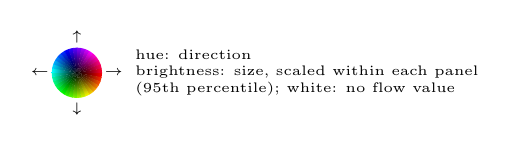
\begin{tikzpicture}[baseline=(wheel.center)]
\node[inner sep=0pt] (wheel) at (0,0) {\phantom{\rule{.7cm}{.7cm}}};
\foreach \a in {0,10,...,350}{%
  \pgfmathsetmacro{\hue}{\a/360}\definecolor{wheelhue}{hsb}{\hue,1,1}%
  \begin{scope}\clip (0,0)--(-\a:.32)--(-\a-11:.32)--cycle;
  \shade[inner color=black,outer color=wheelhue] (0,0) circle (.32);\end{scope}}
\node[font=\tiny,inner sep=1pt] at (0:.47) {$\rightarrow$};\node[font=\tiny,inner sep=1pt] at (-90:.46) {$\downarrow$};
\node[font=\tiny,inner sep=1pt] at (180:.47) {$\leftarrow$};\node[font=\tiny,inner sep=1pt] at (90:.46) {$\uparrow$};
\node[font=\tiny,align=left,anchor=west] at (.62,0) {hue: direction\\brightness: size, scaled within each panel\\(95th percentile); white: no flow value};
\end{tikzpicture}\par\vspace{1mm}
\setlength{\tabcolsep}{3pt}
\begin{tabular}{ccc}
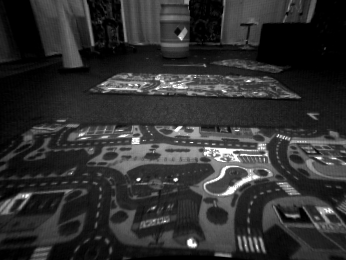
\includegraphics[width=.30\textwidth,height=1.5cm,keepaspectratio]{figures/mvsec_indoor_flying_2_alpha_10_vox_focus/gray_0340.png}&
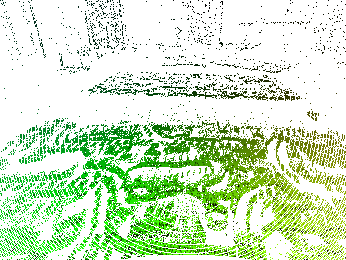
\includegraphics[width=.30\textwidth,height=1.5cm,keepaspectratio]{figures/mvsec_indoor_flying_2_alpha_10_vox_focus/flow_gt_0340.png}&
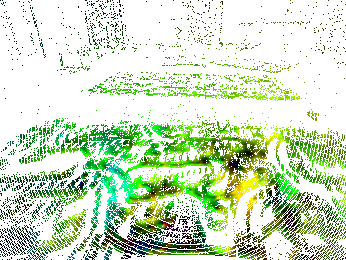
\includegraphics[width=.30\textwidth,height=1.5cm,keepaspectratio]{figures/mvsec_indoor_flying_2_alpha_10_vox_focus/flow_acc_0340.png}\\
Reference&Ground truth&Event-accumulation baseline\\[2mm]
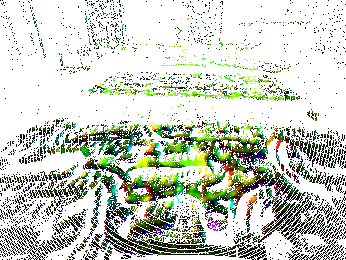
\includegraphics[width=.30\textwidth,height=1.5cm,keepaspectratio]{figures/mvsec_indoor_flying_2_alpha_10_vox_focus/flow_ts_0340.png}&
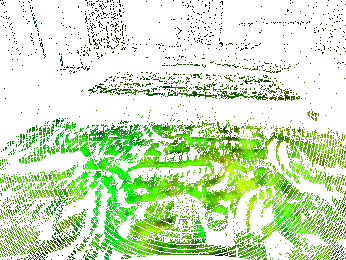
\includegraphics[width=.30\textwidth,height=1.5cm,keepaspectratio]{figures/mvsec_indoor_flying_2_alpha_10_vox_focus/flow_vox_0340.png}&
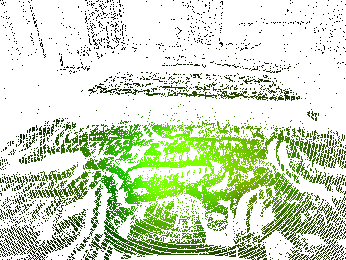
\includegraphics[width=.30\textwidth,height=1.5cm,keepaspectratio]{figures/mvsec_indoor_flying_2_alpha_10_vox_focus/flow_vox_struct_0340.png}\\
Time surface&Voxel&Structure tensor voxel
\end{tabular}
% source detail: Ch. 3, fig:vox\_comparison.
\src{\dref{Figure}{fig:vox_comparison}.}
\talknote{Question: what is the real-data AEE?}{This real-data comparison is qualitative; the AEE values come from the known-motion examples.}{The event-accumulation baseline is a separate comparison method. The theorem's coefficient representations are the time-surface, voxel, and structure-tensor constructions. This is one qualitative example; Chapter 3's AEE values come from the known-motion scenes.}
\end{frame}

\begin{frame}{The quadratic $H^1$ penalty gives a unique, stable flow}
\small
The flow energy uses a quadratic gradient penalty:
% source: Ch. 3 common existence/stability theorem; abstract signed-linear quadratic energy.
\[E(\vct)=\tfrac12\int_\Omega\bigl(\vct^\top\B\vct-2b^\top\vct\bigr)
+\tfrac{\alpha^2}{2}\norm{\nabla\vct}_{L^2}^2,\qquad \vct\in H^1(\Omega;\R^2).\]
% source detail: Ch. 3, thm:unified\_wellposedness, function-space remark, eq:ne\_tensor.
\src{\dref{Theorem}{thm:unified_wellposedness}, function-space remark, \dref{Eq.}{eq:ne_tensor}.}
\talknote{Question: why use $H^1$ instead of TV?}{The quadratic model yields a bilinear form to which Lax--Milgram applies, then an energy identity gives coefficient stability. TV may retain discontinuities, but requires a separate existence framework in $BV$.}{Replacing the gradient term with TV in an abstract signed-linear energy can make it unbounded below. Full-rank pointwise fidelity can retain strict convexity, so TV can keep uniqueness; with TV, $H^1$ coercivity needs more than the integrated condition. TV~\cite{rudin1992nonlinear} preserves jumps and rests on its own $BV$ existence argument with separate uniqueness and stability assumptions. Normalized NE diffusion gives directional quadratic smoothing with a uniform ellipticity floor.}
\end{frame}

\begin{frame}{An MM majorizer matches both the value and the slope}
For a scalar prediction $s$, let $v(s)=|s|+\varepsilon$, $\varepsilon>0$, and
% source: Ch. 4 sec:irls_scope and prop:irls_vs_nll; derivative is direct differentiation away from s=0.
\[S(s)=\frac{(y-s)^2}{2v(s)}+R(s),\qquad
Q_k(s)=\frac{(y-s)^2}{2v(s_k)}+R(s).\]
The frozen surrogate matches $S$ at $s_k$. Away from $s=0$, $S'$ carries the extra term
% source: Ch. 4 sec:irls_scope; derivative of the state-dependent variance term.
\[ -\frac{v'(s)(y-s)^2}{2v(s)^2}.\]
% source detail: Ch. 4, sec:irls\_scope, prop:irls\_vs\_nll; derivative consequence, not a stated MM theorem.
\src{\dref{Section}{sec:thm_foundations}, \dref{Proposition}{prop:irls_vs_nll}; derivative consequence of the proposition.}
\talknote{Question: is this IRLS a majorization-minimization method?}{Only when the derivatives also match. The state-dependent variance contributes the displayed derivative term, which the frozen-weight quadratic omits; a differentiable tangent majorizer must match that derivative as well as the value.}{The proved existence and conditional contraction results concern the fixed-point map. Descent is governed by the implementation's cost-rise acceptance rule, which accepts rises of up to 5\%. A differentiable tangent majorizer matches the derivative at the current iterate; the frozen quadratic matches the value.}
\end{frame}

\begin{frame}{A Gaussian model explains attenuation as evidence}
For common fixed $\Lam\succ0$, $\gamma\ge0$, and independent unit Gaussian noise, the candidate conditional is
% source: supplementary derivation from Ch. 4, prop:correct_selection; P and T are defined there.
\[\mathbf y_R\mid\mathbf y_L\sim\mathcal N(\mathbf c,(2\mathbf P)^{-1}),\qquad
\mathbf c=\mathbf P^{-1}\mathbf T\mathbf y_L.\]
Coupled versus independent evidence satisfies
% source: supplementary Gaussian derivation from Ch. 4 matching-cost decomposition.
\[-\log\frac{p_\gamma(\mathbf y_L,\mathbf y_R)}{p_0(\mathbf y_L,\mathbf y_R)}
=D(\mathbf y_L-\mathbf y_R)+\text{constant}.\]
% source detail: Supplementary Gaussian derivation from Ch. 4, lem:matching\_cost\_closed\_form, prop:correct\_selection.
\src{Supplementary Gaussian derivation from \dref{Lemma}{lem:matching_cost_closed_form}, \dref{Proposition}{prop:correct_selection}.}
\talknote{Question: can attenuation be read probabilistically?}{For fixed common parameters, interpret the magnitude and coupling penalties as a Gaussian prior and observations as independent unit-noise Gaussian measurements. The conditional distribution makes the profile prediction and its uncertainty explicit.}{The prior precision is $\M_0=\left(\begin{smallmatrix}\Lam^2+\gamma I&-\gamma I\\-\gamma I&\Lam^2+\gamma I\end{smallmatrix}\right)$, and $\M=\M_0+\operatorname{diag}(\A,\A)^\top\operatorname{diag}(\A,\A)$. Integrating out the profiles gives $-\log p_\gamma(\mathbf y)=C_\gamma(\mathbf y)+\tfrac12\log\det\M-\tfrac12\log\det\M_0+\text{constant}$; these determinant terms are fixed across candidates. The operator $\mathbf P^{-1}\mathbf T$ has eigenvalues in $[0,1)$ and is self-adjoint and contractive in the $\mathbf P$ metric, but need not contract in Euclidean norm. For scalar $\Lam$, attenuation is diagonal in the temporal observation eigenmodes. The criterion from $D$ alone selects an ideal match for $\gamma>0$, full-row-rank $\A$, and distinct candidate profiles; it is an alternative score. The conditional mean $\mathbf c$ is what explains the attenuation.}
\end{frame}

\begin{frame}{The stereo estimator runs six layers from events to depth}
\begin{tikzpicture}[>=Latex,node distance=4mm,every node/.style={font=\small},box/.style={draw=teal,fill=soft,rounded corners,align=center,text width=3.7cm,minimum height=1cm}]
\node[box] (a) {Rectify, motion-compensate,\\bin and normalize};
\node[box,right=5mm of a] (b) {For each candidate disparity:\\freeze weights, solve, damp};
\node[box,right=5mm of b] (c) {Compute candidate costs\\at returned iterates};
\node[box,below=8mm of c] (d) {Mask, average, normalize,\\aggregate along image paths};
\node[box,left=5mm of d] (e) {Choose disparity;\\interpolate the score minimum};
\node[box,left=5mm of e] (f) {Convert positive valid\\disparity to depth};
\draw[->,thick] (a)--(b);\draw[->,thick] (b)--(c);\draw[->,thick] (c)--(d);\draw[->,thick] (d)--(e);\draw[->,thick] (e)--(f);
\end{tikzpicture}
% source detail: Ch. 4, sec:solution; Appendix, app:protocol\_ch4.
\src{\dref{Section}{sec:solution}; \dref{Section}{app:protocol_ch4}.}
\talknote{Implementation scope; 60 seconds.}{Expand IRLS as iteratively reweighted least squares and SGM as semi-global matching: SGM penalizes disparity changes along multiple paths to encourage spatial coherence. A finite search exactly returns a minimum of the final score list, subject to tie breaking. That exactness is over the computed candidate list.}{Clipping affects solve weights; final scores recompute unclipped weights. Finite penalty sentinels are averaged before selection, so the guidance window is soft. The benchmark includes the finest-level interpolation of the aggregated score but excludes the separate hole-filling/refinement operator. The further analysis distinguishes the optimization and scoring steps explicitly. Theorems describe specific layers; the empirical evaluation describes the complete estimator. The exact minimum of a computed score list certifies the best listed candidate for that score.}
\end{frame}

\begin{frame}{Each problem gets its own mathematical contribution}
\begin{itemize}\setlength{\itemsep}{2mm}
\item \textbf{Images:} temporal inversion with an explicit null space and fixed-weight guarantees.
\item \textbf{Flow:} one well-posedness and stability theorem for three event representations.
\item \textbf{Contrast maximization:} a coercive spline regularizer and a global minimizer.
\item \textbf{Stereo:} block structure, profiled-cost bias, and selection and robustness criteria.
\end{itemize}
% source detail: Chs. 1 and 5; labeled results throughout Chs. 2--4.
\src{\dref{Section}{sec:contribution_matrix} and \dref{Table}{tab:contribution_matrix}.}
\talknote{Question: what is new if the proof tools are classical?}{Credit Tikhonov regularization, Horn--Schunck, Lax--Milgram, and Brouwer as classical tools. Explain the work as constructing and comparing precise event-based inverse models, identifying what assumptions make them well posed, and deriving consequences that are otherwise easy to overclaim. The common flow theorem gives one reusable treatment for all three representations.}{The stereo cost decomposition and attenuation example explain how correct correspondence depends on more than inner solvability. The separation and margin conditions supply a conditional answer. The fixed/adaptive split prevents a quadratic guarantee from being incorrectly transferred to a changing-weight procedure. These are concrete mathematical insights that inform model design and evaluation. Classical proof tools connect the models; the event-specific formulations, hypotheses, consequences, and limits are the research content. Stereo also has a scoped adaptive-weight analysis.}
\end{frame}

\begin{frame}{Literature anchors and where to find the claims}
\begin{columns}[T]
\column{.48\textwidth}\footnotesize
\textbf{Image reconstruction}
\begin{itemize}
% source: Rebecq et al., CVPR 2019, Events-to-Video, primary paper.
% link: https://openaccess.thecvf.com/content_CVPR_2019/papers/Rebecq_Events-To-Video_Bringing_Modern_Computer_Vision_to_Event_Cameras_CVPR_2019_paper.pdf
\item \textcolor{teal}{Rebecq et al.}~\cite{rebecq2019events}\\\emph{Events-to-Video}.
% source: Zhang, Yezzi, and Gallego, TPAMI 2023; doi:10.1109/TPAMI.2022.3230727.
% link: https://arxiv.org/abs/2112.06242
\item \textcolor{teal}{Zhang, Yezzi \& Gallego}~\cite{zhang2021formulating}\\\emph{Image reconstruction as a linear inverse problem using optical flow}.
% source: Antil and Sayre, Inverse Problems 2023; doi:10.1088/1361-6420/ace7c7.
% link: https://arxiv.org/pdf/2302.02052
\item \textcolor{teal}{Antil--Sayre}~\cite{HAntil_DSayre_2023a}\\\emph{Bilevel inverse problems in neuromorphic imaging}.
\end{itemize}
\textbf{Sensor overview}
% source: Gallego et al., TPAMI 2022; doi:10.1109/TPAMI.2020.3008413.
\par\smallskip\textcolor{teal}{Gallego et al.}~\cite{gallego2022event}: \emph{Event-Based Vision: A Survey}.
\column{.49\textwidth}\footnotesize
\textbf{Flow models and analysis}
\begin{itemize}
% source: Horn and Schunck, Artificial Intelligence 1981, primary author-hosted paper.
% link: https://people.csail.mit.edu/bkph/papers/Optical_Flow_OPT.pdf
\item \textcolor{teal}{Horn--Schunck}~\cite{horn1981determining}\\\emph{Determining Optical Flow}.
% source: Benosman et al., TNNLS 2014; doi:10.1109/TNNLS.2013.2273537.
\item \textcolor{teal}{Benosman et al.}~\cite{benosman2014event}\\\emph{Event-Based Visual Flow}.
% source: Weickert and Schnorr, IJCV 2001; doi:10.1023/A:1013614317973.
\item \textcolor{teal}{Weickert--Schn\"orr}~\cite{weickert2001theoretical}\\\emph{Convex regularizers for image motion}.
% source: Gallego, Rebecq, and Scaramuzza, CVPR 2018; dissertation bibliography gallego2018unifying.
% link: https://arxiv.org/abs/1804.01306
\item \textcolor{teal}{Gallego, Rebecq \& Scaramuzza}~\cite{gallego2018unifying}\\\emph{A Unifying Contrast Maximization Framework}.
\end{itemize}
\textbf{Evaluation data}
% source: Zhu et al., RA-L 2018; doi:10.1109/LRA.2018.2800793.
\par\smallskip\textcolor{teal}{Zhu et al.}~\cite{MVSEC2018}: \emph{The Multivehicle Stereo Event Camera Dataset}.
\end{columns}
% source detail: Ch. 2 and Ch. 3 related work; Appendix evaluation protocol. Links identify primary sources; the companion reference notes give full titles and comparison scope.
\src{\dref{Chapter}{ch:monocular_reconstruction}; \dref{Section}{sec:related_work}; \dref{Section}{app:protocol_ch4}. Numbers match the dissertation bibliography; full entries on the closing reference pages.}
\talknote{Attribution.}{The reconstruction references distinguish learned event-only video reconstruction, flow-based image inversion, and frame-assisted bilevel deblurring. The flow references identify the classical variational structure, timestamp geometry, existing well-posedness theory, and nonconvex contrast maximization.}{The dissertation's contribution is the stated event-derived models, shared coefficient analysis, and derived conditioning, bias, and selection consequences. The presentation's empirical values and theorem statements come from the dissertation. The source map ties each slide to its relevant labels, figures, and tables.}
\end{frame}

\begin{frame}{The error splits into regularization bias and noise}
For fixed scalar $\lambda>0$, $\mathbf y=\A\mathbf f^\dagger+\boldsymbol\eta$, and $\K=\A^\top\A+\lambda^2\mathbf I$,
% source: Ch. 2 thm:uniqueness, prop:stability; bias-noise split follows by direct substitution.
\[\mathbf f_\lambda-\mathbf f^\dagger
=-\lambda^2\K^{-1}\mathbf f^\dagger+\K^{-1}\A^\top\boldsymbol\eta.\]
The two terms are regularization bias and propagated observation noise.
% source detail: Ch. 2, thm:uniqueness, prop:stability; direct bias-noise identity.
\src{\dref{Theorem}{thm:uniqueness}, \dref{Proposition}{prop:stability}; direct bias-noise identity.}
\talknote{Question: does stability imply truth?}{No. The estimator's error splits into a shrinkage bias and propagated noise. The stability bound controls sensitivity to the observations, while the bias depends on the signal and the penalty.}{A zero-mean reference fixes the unobservable constant ambiguity. On a fixed grid, noiseless data from a mean-zero reference signal are recovered as $\lambda\to0$. Persistent noise can prevent recovery as $\lambda\to0$; uniform refinement requires controlling noise, regularization, and grid scaling. Model error may enter the residual separately from sensor noise. Stability controls sensitivity to the data; accuracy is a separate property.}
\end{frame}

\begin{frame}{Sub-threshold signals share one empty event stream}
The binned increment matrix has $\ker\A=\operatorname{span}\{\mathbf1\}$. The ideal sensor also maps distinct time-varying signals to one stream:
% source: Ch. 2 eq:polarity; zero-event pair below is a direct ideal-threshold illustration.
\[L_1(t)=L_0,\qquad L_2(t)=L_0+a\sin(2\pi t/T),\qquad
0<a<c_{\rm th},\quad t\in[0,T].\]
Both start at $L_0$, emit no events, and have positive intensities $I_j(t)=e^{L_j(t)}$.
% source detail: Ch. 2, eq:polarity, lem:nullspace; direct ideal-sensor example.
\src{\dref{Eq.}{eq:polarity}, \dref{Lemma}{lem:nullspace}; direct ideal-sensor example.}
\talknote{Question: is the constant nullspace the whole sensor ambiguity?}{No. The chain matrix has exactly the constant nullspace, but the sensor only fires after a contrast threshold crossing. The two displayed positive intensity signals share the same initial reference and remain inside that threshold, so both produce the same empty event stream.}{This example shows that a physical stream can omit changes that never cross threshold. A small perturbation supported strictly away from existing crossings can preserve that schedule when there is a positive threshold margin. The chain null space describes the discrete increment surrogate; the physical sensor adds sub-threshold ambiguity.}
\end{frame}

\begin{frame}{Integrated directional information is necessary for uniqueness}
Let $\Omega$ be connected, bounded, and Lipschitz; $\alpha>0$; $\B\in L^\infty$ symmetric PSD; and $b\in L^2$. Minimize over unrestricted $H^1(\Omega;\R^2)$ fields. Set $M_B=\int_\Omega\B$.
% source: Ch. 3 thm:unified_wellposedness; the converse follows directly for its quadratic energy.
If $M_B$ is singular, choose $c\ne0$ with $M_Bc=0$. Then $\B c=0$ a.e. and
\[E(\vct+tc)=E(\vct)-t\,c^\top\!\int_\Omega b.\]
If the coefficient is nonzero, $E$ is unbounded below; if zero, it is flat in direction $c$.
% source detail: Ch. 3, thm:unified\_wellposedness; direct converse for its quadratic energy.
\src{\dref{Theorem}{thm:unified_wellposedness}; direct converse for its quadratic energy.}
% source: Ch. 3 thm:unified_wellposedness; PSD plus zero integral of c^T B c forces Bc=0 a.e.
\talknote{Question: why require $\int\B\succ0$?}{A singular integrated matrix leaves a nonzero constant flow direction unseen by both the data quadratic and the gradient penalty. Along that direction, the remaining linear term either drives the energy without a lower bound or vanishes.}{Because $\B$ is PSD, $c^\top\B(x)c\ge0$ a.e.; its integral is $c^\top M_Bc=0$, so $\B^{1/2}c=0$ and hence $\B c=0$ a.e. In the zero-slope case, any existing minimizer would have a flat family, so uniqueness fails; existence needs a separate argument. Residual-square data can make the linear coefficient compatible with the null direction. Boundary constraints or a ridge term change the argument.}
\end{frame}

\begin{frame}{Coefficient stability is one stage of event-to-flow stability}
\centering
\begin{tikzpicture}[>=Latex,node distance=7mm,every node/.style={draw=teal,fill=soft,rounded corners,align=center,text width=3.4cm,minimum height=1cm}]
\node (a) {Event stream $E$};
\node[right=of a] (b) {Representation and fitted coefficients $(\B,b)$};
\node[right=of b] (c) {Estimated flow $v^*$};
\draw[->,thick] (a)--(b);\draw[->,thick] (b)--(c);
\end{tikzpicture}
\par
% source: Ch. 3 thm:unified_wellposedness and prop:ts_regression_bound; composition is a scope observation.
\vspace{4mm}
The theorem bounds the second arrow. A Lipschitz representation map composes with it.
% source detail: Ch. 3, thm:unified\_wellposedness, prop:ts\_regression\_bound; supplementary scope explanation.
\src{\dref{Theorem}{thm:unified_wellposedness}, \dref{Proposition}{prop:ts_regression_bound}; supplementary scope explanation.}
% source: supplementary metric illustration for one positive unit atom; total variation norm uses measure variation.
\talknote{Question: how stable is the full event-to-flow pipeline?}{The variational theorem begins after events have become coefficient fields. If preprocessing were Lipschitz in a chosen event metric, its bound could compose with the coefficient-to-flow estimate.}{The metric matters: moving one positive unit atom by nonzero $\delta t$ gives the total variation norm $\lVert\delta_{t+\delta t}-\delta_t\rVert_{\rm TV}=2$, while the single-atom mass-one Wasserstein distance is $|\delta t|$. Hard bins or changing candidate neighborhoods may jump; fixed-bandwidth smoothing can behave better under a suitable metric. An end-to-end guarantee adds a metric and a stability result for the event preprocessing.}
\end{frame}

\begin{frame}{Matching a continuum objective sets the penalty's grid scaling}
\small
Smooth, uniform-time model: spacing $h$, increments $y_i=h g_i$, and target energy
% source: Ch. 2 eq:tempdiffA, eq:in; continuum quadrature scaling is a supplementary derivation.
\[\frac12\int|f'-g|^2dt+\frac{\beta_{\rm time}^2}{2}\int|f|^2dt
\quad\leadsto\quad
\frac1{2h}\norm{\A f-y}^2+\frac{\beta_{\rm time}^2h}{2}\norm{f}^2.\]
Multiplying the discrete objective by $h$ gives the Chapter 2 form with
% source: direct coefficient matching to Ch. 2 eq:in.
\[\lambda_h=\beta_{\rm time}h.\]
% source detail: Ch. 2, eq:tempdiffA, eq:in; supplementary smooth-model scaling illustration.
\src{\dref{Eq.}{eq:tempdiffA}, \dref{Eq.}{eq:in}; supplementary smooth-model scaling illustration.}
\talknote{Question: should $\lambda$ change as the grid is refined?}{The answer depends on the target continuum functional. In this smooth uniform-time illustration, difference residuals scale like $h$, while the Riemann sum contributes $1/h$. Matching the magnitude penalty yields $\lambda_h=\beta_{\rm time}h$.}{Finite-endpoint quadrature may need endpoint weights. A physical event model would also require a scaling choice for noise and kernel bandwidth. The penalty's grid scaling follows the continuum objective being approximated; this is an illustrative model.}
\end{frame}

\begin{frame}{Strong smoothness selects one constant flow}
For fixed $\Omega,\B,b$ satisfying the unified theorem, with unrestricted $H^1$ fields and the same $\alpha^2$ gradient coefficient,
% source: Ch. 3 thm:unified_wellposedness; the alpha-to-infinity limit is a direct corollary derivation.
\[\alpha\to\infty\quad\Longrightarrow\quad
v_\alpha\to c\text{ in }H^1,\qquad
c=\left(\int_\Omega\B\right)^{-1}\int_\Omega b.\]
% source detail: Ch. 3, thm:unified\_wellposedness; direct strong-regularization limit.
\src{\dref{Theorem}{thm:unified_wellposedness}; direct strong-regularization limit.}
% source: Ch. 3 thm:unified_wellposedness; direct estimate from its weak equation and Poincare inequality.
\talknote{Question: what happens as $\alpha$ grows?}{The gradient penalty forces the minimizer toward a constant field. The data term then selects the constant that balances the integrated directional information against the integrated forcing.}{For a proof, write $w_\alpha=v_\alpha-c$ and test the weak equation with it. With $h_b=b-\B c$ and $\int h_b=0$, the identity is $\int w^\top\B w+\alpha^2\norm{\nabla w}_2^2=\int h_b\cdot(w-\bar w)$. Poincare gives $\norm{\nabla w}=O(\alpha^{-2})$. Testing constants yields $\int\B w=0$; positive definiteness of $\int\B$ and Poincare then give $\bar w\to0$. This is a direct corollary.}
\end{frame}

\begin{frame}{Density conservation adds a compression term}
Scalar transport and source-free density conservation are
% source: Ch. 3 subsec:vox_projection and sec:vox_cont_exclusion; product rule is direct.
\[V_t+v\cdot\nabla V=0,\qquad
V_t+\nabla\cdot(Vv)=0,\qquad
\nabla\cdot(Vv)=v\cdot\nabla V+V\,\nabla\cdot v.\]
They coincide when $V\nabla\cdot v=0$, in particular for divergence-free flow.
% source detail: Ch. 3, subsec:vox\_projection, sec:vox\_cont\_exclusion; direct product-rule comparison.
\src{\dref{Section}{subsec:vox_projection}, Scalar transport and density conservation (\drefpage{sec:vox_cont_exclusion}); direct product-rule comparison.}
% source: Ch. 3 sec:vox_cont_exclusion; one-dimensional v=x, V=1 is a direct illustration.
\talknote{Question: should events be modeled as a conserved fluid?}{That is an additional physical assumption. Scalar transport follows a pattern value along a trajectory; density conservation also accounts for compression or expansion through the divergence of flow.}{For a simple illustration, in one dimension let $v(x)=x$ and $V(x,t)=1$. It solves scalar transport, but source-free conservation has residual $\partial_x(Vv)=1$. A source term $V_t+\nabla\cdot(Vv)=s$ may be appropriate if events are created or lost.}
\end{frame}

\begin{frame}{Correlated errors change the regression uncertainty}
For a centered symmetric regression design $Z$ with $Q=Z^\top Z\succ0$, timestamp-error covariance $\Sigma$ gives
% source: Ch. 3 prop:ts_regression_bound; covariance identity is the direct OLS extension to correlated errors.
\[\operatorname{Cov}(\hat g)=Q^{-1}Z^\top\Sigma ZQ^{-1}.\]
This reduces to $\sigma^2Q^{-1}$ when $\Sigma=\sigma^2 I$.
\par\medskip
% source: Ch. 2 eq:in and thm:uniqueness; positive definite fidelity matrix preserves SPD.
With any $\Gamma\succ0$, the temporal system matrix is $\A^\top\Gamma^{-1}\A+\Lam^2\succ0$ when $\Lam\succ0$.
% source detail: Ch. 3, prop:ts\_regression\_bound; Ch. 2, eq:in, thm:uniqueness; direct correlated-error extension.
\src{\dref{Proposition}{prop:ts_regression_bound}; \dref{Eq.}{eq:in}, \dref{Theorem}{thm:uniqueness}; direct correlated-error extension.}
% source: direct OLS linear-map covariance; Ch. 2 thm:uniqueness for weighted SPD normal matrix.
\talknote{Question: what if timestamp errors are correlated?}{The covariance formula of a linear OLS estimator holds for correlated errors; the full covariance matrix replaces the white-noise simplification. If each error has the same mean, the centered symmetric design cancels that mean in the slope.}{Smoothing errors with $H_\epsilon$ produces $H_\epsilon\Sigma H_\epsilon^\top$, which may be singular; check its rank before inverting. A positive definite fidelity precision $\Gamma^{-1}$ keeps the regularized normal matrix positive definite, but changes coefficients and constants. A Gaussian likelihood interpretation needs a separate distributional assumption.}
\end{frame}

\begin{frame}{Optical flow: further analysis}
\hypertarget{flowdetails}{}
\begin{itemize}
\item Time-surface gradient estimation: bias, variance, and design.
\item Contrast maximization: what it models, known-motion evidence, objective, existence proof, and comparison with the voxel models.
\end{itemize}
\vspace{2mm}
Regression quantifies coefficient uncertainty; contrast maximization changes the objective being optimized.
\talknote{Divider for questions.}{Use when asked how time-surface gradients are estimated, or about contrast maximization, the most widely used event-based motion objective.}{Contrast maximization answer in one sentence: a global minimizer exists by finite-dimensional coercivity with the coefficient ridge; the local solver carries no global guarantee.}
\end{frame}

\begin{frame}{Larger fitting disks trade variance for curvature bias}
\small
Fit a plane to timestamps at offsets $\mathbf z_j$ around a pixel.
\[Q=\sum_j\mathbf z_j\mathbf z_j^\top\succ0.\]
For a centrally symmetric design and independent timestamp errors with common mean and finite variance $\sigma^2$:
\[\operatorname{Cov}(\widehat{\nabla\mathcal T})=\sigma^2 Q^{-1}.\]
With a Lipschitz Hessian of constant $L_H$ on a neighborhood containing the sample disk,
% source: Ch. 3 prop:ts_regression_bound(iv), eq:ts_discrete_bias and eq:ts_discrete_mse; L_H renames its Lipschitz constant L.
\[\norm{\operatorname{Bias}}\le\frac{L_H}{6}\norm{Q^{-1}}\sum_j\norm{\mathbf z_j}^4,\qquad
\operatorname{MSE}=\norm{\operatorname{Bias}}^2+\sigma^2\operatorname{tr}(Q^{-1}).\]
% source detail: Ch. 3, prop:ts\_regression\_bound.
\src{\dref{Proposition}{prop:ts_regression_bound}.}
\talknote{Gradient-estimation result; 75 seconds; shorten to the takeaway in a compressed talk.}{The design matrix Q depends only on sample positions. Central symmetry decouples the intercept and cancels the quadratic Taylor term in the slope. A Lipschitz Hessian leaves a cubic remainder bounded by L\_H |z|\textasciicircum{}3/6. Multiplication by z and Q\textasciicircum{}{-1} yields the bias bound. Independent equal-variance errors give the covariance, and the MSE decomposition combines both contributions for the same discrete estimator.}{A full-rank disk of timestamps around a moving straight edge can estimate its gradient well while the tangential velocity remains unidentified. The timestamp-noise model is an assumption of the theorem. The asymptotic radius heuristic is in the backup, with its finite-design qualifications. Regression rank and velocity identifiability are different questions.}
\end{frame}

\begin{frame}{CMAX has the lowest error in every known-motion scene}
\centering\vfill
% source: ../dissertation_thesis/shared_bodies/ch3_eb_hs_of_body.tex fig:ch3_quiver_synth and fig:ch3_quiver_v2e (figures/ch3_quivers_consistent/manifest.tsv, aee_at_frame, 2 d.p.).
\renewcommand{\arraystretch}{1.4}\begin{tabular}{@{}lcc@{}}\toprule
AEE (px) & Structure tensor & CMAX\\\midrule
% source: fig:ch3_quiver_synth AEE row: vox_struct 2.15, cmax 0.49.
Idealized stripes & 2.15 & \textbf{0.49}\\
% source: fig:ch3_quiver_v2e AEE rows: v2e_stripes vox_struct 1.92, cmax 1.19; v2e_checker vox_struct 0.98, cmax 0.32.
Simulated stripes (v2e) & 1.92 & \textbf{1.19}\\
Simulated checkerboard (v2e) & 0.98 & \textbf{0.32}\\\bottomrule
\end{tabular}\par\medskip
{\small\color{muted}Window 22; a zero flow field scores 3.00\,px. The structure tensor is the best quadratic model.\par}
\vfill
% source detail: Ch. 3, sec:cmax introduction (binning blur), fig:ch3_quiver_synth, fig:ch3_quiver_v2e.
\src{\dref{Section}{sec:cmax}; \dref{Figure}{fig:ch3_quiver_synth} and \dref{Figure}{fig:ch3_quiver_v2e}; contrast maximization~\cite{gallego2018unifying,shiba2022secrets}; v2e~\cite{hu2021v2e}.}
% source: AEE gaps 2.15-0.49=1.66, 1.92-1.19=0.73, 0.98-0.32=0.66 from fig:ch3_quiver_synth/fig:ch3_quiver_v2e; normal-flow reference 3/sqrt(2)=2.12 px from Ch. 3 known-motion discussion.
\talknote{What CMAX models and why it is promising; 60 seconds.}{Describe the warp in scene terms: the right motion turns a smeared trail into a sharp edge. The quadratic models first compress events into a time surface or bins and fit coefficients; CMAX keeps each event's own time. In all three known-motion scenes its AEE is the lowest, by 0.66 to 1.66 px over the structure tensor. On the stripes it recovers the diagonal, where interior pixels alone determine only the across-stripe component (normal-flow reference error 2.12 px).}{Scope: one representative window (chosen by the median-deviation rule) on simulated scenes with known motion. On the idealized stripes CMAX also assigns flow to the surrounding background. The dissertation's AEE values come from the known-motion scenes. Its guarantee is existence of a global minimizer; the quasi-Newton solver is local. After the protocol slide come the objective, the existence proof, and a comparison with the voxel models. CMAX keeps each event's own time; binned models blur when an edge moves during a bin. On the stripes, the warp brings in the object's boundary, so CMAX recovers the diagonal.}
\end{frame}

\begin{frame}[t,label=flowprotocol]{Every method sees the same motion, window, and arrow scale}
\footnotesize\renewcommand{\arraystretch}{1.15}
\begin{tabular}{p{.20\textwidth}p{.71\textwidth}}
\toprule Aspect & Reported protocol\\\midrule
% source: Ch. 3 known-motion comparison, line 1058.
Stimulus & A $60\times40$ px object translates diagonally at $3$ px per window; direct idealized events and v2e-simulated events~\cite{hu2021v2e}.\\
% source: Ch. 3 known-motion comparison, line 1058; the 100-iteration cap belongs to these figures, not the separate MVSEC run.
Settings & Quadratic variants: $\alpha_{\rm smooth}=20$, single scale. Contrast maximization: $100$ L-BFGS~\cite{zhu1997algorithm} iterations.\\
% source: Ch. 3 known-motion window-selection rule, line 1060.
Selection & Window $22$ minimizes summed deviation from each variant's median AEE over windows $1$--$31$.\\
Display / error & Common arrow scale; AEE is mean Euclidean displacement error, in pixels per evaluation window.\\\bottomrule
\end{tabular}
\src{\dref{Figure}{fig:ch3_quiver_synth} and \dref{Figure}{fig:ch3_quiver_v2e}; smoothing stencils (\drefpage{app:ch3_discrete_stencils}).}
\talknote{Question: how were the examples selected, and how fair is the comparison? About 90 seconds.}{State the motion and event generators, the shared display scale, the selection rule, and AEE units. The zero-field reference has error equal to the displacement magnitude. The settings describe the evaluated implementations; the same numerical alpha gives each implementation its own effective smoothing and computational work.}{The appendix distinguishes an eight-neighbor VOX stencil from a four-neighbor structure-tensor stencil. The separate MVSEC contrast-maximization protocol has a different iteration cap. The evaluation mask is denoted by M in the cited passage; use the cited definition. Use existing real-data and CMAX backups for generalization and optimization questions. Equal numerical $\alpha$ values give different stencil-dependent smoothing strengths. These controlled examples show directional-information effects at the reported solver settings.}
\end{frame}

\begin{frame}{Contrast maximization sharpens the warped event image}
\begin{columns}[c]
\column{.42\textwidth}\centering
\begin{tikzpicture}[x=1.05cm,y=.78cm,>=Latex]
\draw[->,muted] (0,0)--(3.2,0) node[right,font=\scriptsize]{$x$};
\draw[->,muted] (0,0)--(0,2.4) node[above,font=\scriptsize]{$\tilde t$};
\draw[dashed,muted] (0,1.1)--(3.0,1.1) node[right,font=\scriptsize]{$\tilde t_{\rm ref}$};
\draw[dotted,teal,thick] (1.7,0)--(1.7,2.2);
\foreach \t in {.2,.65,1.55,2.0}{\draw[teal,thick,->,shorten >=2pt] ({.6+\t},\t)--(1.7,\t);}
\foreach \t in {.2,.65,1.1,1.55,2.0}{\fill[evpos] ({.6+\t},\t) circle (2.4pt);}
\node[left,font=\scriptsize] at (0,-.75) {$\mathbf q=0$};
\foreach \x in {.8,1.25,1.7,2.15,2.6}{\fill[muted] ({\x-.07},-1.0) rectangle ({\x+.07},-.72);}
\draw[muted] (0,-1.0)--(3.0,-1.0);
\node[left,font=\scriptsize] at (0,-1.75) {correct $\mathbf q$};
\fill[teal] (1.63,-2.3) rectangle (1.77,-1.15);
\draw[muted] (0,-2.3)--(3.0,-2.3);
\end{tikzpicture}
\column{.56\textwidth}
{\color{teal}\textbf{1. Warp}} each event to $\tilde t_{\rm ref}$
\[\mathbf x_k^w=\mathbf x_k+(\tilde t_{\rm ref}-\tilde t_k)\,\mathbf q(\mathbf x_k)\]
{\color{teal}\textbf{2. Accumulate}} them into an image $I_{\mathbf c}$\par\medskip
{\color{teal}\textbf{3. Sharpen}}
\[\min_{\mathbf c}\;-\operatorname{Var}(I_{\mathbf c})+R(\mathbf c)\]
{\small\color{muted}$\mathbf q$: cubic B-spline with coefficients $\mathbf c$;\\ $R$: anisotropic smoothness $+$ a small ridge\par}
\end{columns}
% source detail: Ch. 3, sec:cmax, subsec:cmax_energy, eq:cmax_energy, eq:cmax_ridge_K; app:ch3_cmax_params (h = 8 px cubic B-splines; ON events w_k = 1; reference time at the window midpoint).
\src{\dref{Section}{sec:cmax}, \dref{Eq.}{eq:cmax_energy}, \dref{Eq.}{eq:cmax_ridge_K}; parameters \drefpage{app:ch3_cmax_params}; contrast maximization~\cite{gallego2018unifying}.}
\talknote{Representation and objective; about 75 seconds.}{Left: one edge's events in the $(x,\tilde t)$ plane lie along a slanted line. With zero flow they land at five places, a smeared trail; warping each one by $(\tilde t_{\rm ref}-\tilde t_k)\mathbf q$ moves them to one column, a single tall bar. Right, step 1: the warp uses each event's own time, with $\mathbf q$ a displacement per normalized window, represented by a cubic B-spline with coefficients $\mathbf c$. Step 2: bilinear accumulation gives the warped-event image $I_{\mathbf c}$, which changes as $\mathbf c$ changes. Step 3: maximize its variance, written as minimizing $-\operatorname{Var}$, plus a quadratic regularizer on the coefficients.}{Conventions: $\tilde t=(t-t_0)/T$; $\mathbf q=T\vct_{\rm phys}$ in pixels per window; cubic B-splines with knots every 8\,px; only ON events, $w_k=1$; $\tilde t_{\rm ref}$ at the window midpoint. In full, $R(\mathbf c)=\mathbf c^\top\K_{\rm reg}\mathbf c$ with $\K_{\rm reg}=\beta(\mathbf I_2\otimes\K_{\rm stiff}(\mathbf D))+\tau_{\rm ridge}\mathbf I$ and $\mathbf D=\alpha_{\rm ani}^2\mathbf J_{\sigma_\rho}+\varepsilon_{\rm ell}\mathbf I$. Stiffness penalizes nonconstant splines, most across event edges; the ridge, $\tau_{\rm ridge}=2\varepsilon_{\rm ridge}/M$, controls constant flow and supplies coercivity. Splines give point values at events. The focus term is nonconvex; a wrong warp can raise variance by collapsing events~\cite{shiba2022secrets}.}
\end{frame}

\begin{frame}{The contrast objective has a global minimizer}
\small
For finitely many fixed event weights, let $W_{\rm tot}=\sum_k|w_k|$.
The bilinear accumulation is continuous and satisfies
\[\operatorname{Var}(I_{\mathbf c})\le\frac{W_{\rm tot}^2}{HW}.\]
Therefore
\[F(\mathbf c)\ge-\frac{W_{\rm tot}^2}{HW}+\tau_{\rm ridge}\norm{\mathbf c}^2\longrightarrow\infty.
\]
\begin{block}{Proof mechanism}
Continuous objective $+$ bounded focus gain $+$ coercive ridge\quad$\Rightarrow$\quad compact sublevel set\quad$\Rightarrow$\quad Weierstrass.
\end{block}
% source detail: Ch. 3, prop:cmax\_existence and evaluated-solver scope.
\src{\dref{Proposition}{prop:cmax_existence} and evaluated-solver scope.}
\talknote{Existence proof; 75 seconds.}{A bilinear tent contribution is a continuous function of the warped event location, including when a location crosses a pixel boundary. Each event distributes at most its absolute weight onto the canvas, so the image L1 norm and maximum absolute entry are at most W\_tot. Bound variance by the second moment, then by max times L1 divided by the number of pixels.}{The negative focus term is bounded below. The positive coefficient ridge drives the energy to infinity as the coefficient norm grows, so a global minimizer exists by Weierstrass. This is a finite-dimensional existence result; uniqueness and convergence of the local solver remain open. The evaluated tent objective is only piecewise differentiable, and the solver returns a local solution. The ridge eigenvalue $2\varepsilon/M$ shrinks under refinement in coefficient space; as a function-space penalty it is a uniform $L^2$ term (Backup 69, page 102).}
\end{frame}

\begin{frame}{Voxel models and CMAX combine events at different stages}
\vfill
\small\renewcommand{\arraystretch}{1.6}
\begin{tabular}{@{}>{\raggedright\arraybackslash}p{2.6cm}>{\centering\arraybackslash}p{4.8cm}>{\centering\arraybackslash}p{4.8cm}@{}}
\toprule
 & {\color{teal}\textbf{Voxel projection,\newline structure tensor}} & {\color{amber}\textbf{Contrast maximization}}\\\midrule
Events combined & before the solve, into fixed $\B,b$ & during the solve, after each warp\\
Data term & per pixel: $\vct^\top\B\vct-2b^\top\vct$ & whole image: $-\operatorname{Var}(I_{\mathbf c})$\\
Problem & quadratic, convex & nonconvex\\
Guarantee & unique minimizer if $\int_\Omega\B\succ0$ & a global minimizer exists\\
Solver & Jacobi sweeps, convergent & L-BFGS-B, local\\\bottomrule
\end{tabular}
\vfill
% source detail: Ch. 3, sec:cmax (volume flattening vs. per-event warp), thm:unified_wellposedness, thm:convergence, prop:cmax_existence, app:ch3_cmax_params (L-BFGS-B).
\src{\dref{Theorem}{thm:unified_wellposedness}; \dref{Theorem}{thm:convergence}; \dref{Section}{sec:cmax}; \dref{Proposition}{prop:cmax_existence}.}
\talknote{Comparison; about 75 seconds.}{Read the rows top to bottom; the two voxel models share a column because they agree on every row except the data term. Both voxel models turn events into fixed coefficients before solving, so any motion inside a bin or window is already averaged into $\B$ and $b$. Contrast maximization keeps each event's own time and re-forms the image at every candidate flow. That is why its data term covers the whole image instead of one pixel at a time, and why the problem leaves the quadratic family.}{What each side gets for it: the voxel models get uniqueness under a condition the scene supplies, stability in the coefficients, and a convergent iteration; contrast maximization gets each event's own timing and the lowest known-motion error (Backup 43), with existence of a global minimizer and a local solver. The structure tensor also enters contrast maximization through its regularizer: $\mathbf D$ is built from the event structure tensor. Further rows if asked: the voxel models solve for $\vct$ at every pixel in $H^1$, CMAX for spline coefficients $\mathbf c$; voxel projection assumes one $\vct$ over the window, the structure tensor one $\vct$ across the neighborhood, CMAX moves each event by $\mathbf q(\mathbf x_k)$ per window; the voxel minimizer is also stable in $\B,b$. The time surface sits in the quadratic family with the voxel models: its column reads like voxel projection's, with data term $(\nabla\mathcal T\cdot\vct-1)^2$.}
\end{frame}

\begin{frame}{Stereo depth: full Chapter 4 arc}
\hypertarget{stereoarc}{}
\begin{enumerate}\small
\item Coupled model and the frozen-weight inner solve.
\item Sum and difference modes; the profiled candidate cost.
\item The explicit counterexample and the correct-selection theorem.
\item Winning-margin stability and the non-identifiability example.
\item Heteroscedastic weights and IRLS fixed-point analysis.
\item MVSEC benchmark, weighting comparison, and hard fusion.
\end{enumerate}
\vspace{1mm}
These results separate the inner temporal solve from the outer correspondence decision.
\talknote{Divider for questions; the full stereo arc runs about 17 minutes if presented in sequence.}{Choose the page that matches the question. For ``does the correct disparity win?'', go to the counterexample and then the selection theorem. For ``does IRLS converge?'', go to the fixed-point slide and its backup proof.}{The next page summarizes the four results these pages prove; the core talk shows the model, the inner solve, and the MVSEC table.}
\end{frame}

\begin{frame}{What Chapter 4 adds to stereo depth}
\footnotesize
At each candidate disparity $d$, solve two coupled temporal profiles:
\[\min_{\fL,\fR}\ \sum_{c=L,R}\Bigl(\tfrac12\norm{\W_c^{1/2}(\A\mathbf f_c-\mathbf y_c)}^2+\tfrac12\norm{\Lam\mathbf f_c}^2\Bigr)+\tfrac\gamma2\norm{\fL-\fR}^2.\]
\vspace{-3mm}
\begin{enumerate}\setlength{\itemsep}{0pt}
\item \textbf{Inner solve.} The Hessian is $\succeq\lambda_{\min}^2\mathbf I$, so every candidate has one minimizer.
% source: Ch. 4 lem:matching_cost_closed_form, prop:attenuation_bias; exact example C(1)=1/3, C(1/2)=9/40.
\item \textbf{Profiled cost.} $C(d)=m(\yL)+m(\yR(d))+D_d$: an attenuated copy can outscore the true match ($\tfrac9{40}$ vs.\ $\tfrac13$).
\item \textbf{Selection.} A separation condition makes the correct candidate win; a margin $\Delta$ tolerates perturbations below $\Delta/2$.
\item \textbf{Reweighting.} The IRLS map has a fixed point (Brouwer) and contracts under a sufficient condition.
\end{enumerate}
% source: appendix_bodies/ch4_protocol.tex tab:unified_benchmark and following paragraph: WLS best on Fl2 (58.35) and log RMSE x100 (44.54), second-best elsewhere; 2.66M vs Piatkowska 1.20M points.
MVSEC indoor flying: soft-coupled WLS is best on Flying 2 (58.35\,cm) and log RMSE $\times100$ ($44.54$), second elsewhere, with 2.66\,M scored points versus 1.20\,M for the strongest prior method.
% source detail: Ch. 4, thm:weighted\_spd, prop:attenuation\_bias, prop:correct\_selection, prop:irls\_contraction; App., tab:unified\_benchmark.
\src{\dref{Theorem}{thm:weighted_spd}, \dref{Proposition}{prop:attenuation_bias}, \dref{Proposition}{prop:correct_selection}, \dref{Proposition}{prop:irls_contraction}; \dref{Table}{tab:unified_benchmark}; MVSEC~\cite{MVSEC2018}, Piatkowska~\cite{piatkowska2017}, Brouwer~\cite{brouwer1911beweis}.}
\talknote{Question: what are the Chapter 4 results? About 2 minutes; the four results and one benchmark sentence.}{This chapter compares candidate correspondences by reconstructing and softly coupling a temporal event-feature profile from each view. The analysis separates the unique inner reconstruction from the outer correspondence decision, then gives conditions for selection and stability under a positive winning margin. Item 1 is the Chapter 2 coercivity argument with one more nonnegative term. Item 2 is the conceptual point: after profiling out the latent profiles, the candidate cost contains a right-view monocular term that changes with the candidate, so in the two-sample example an attenuated wrong match beats the exact match. Item 3 gives a sufficient condition under which the correct candidate wins, and its stability under perturbations smaller than half the margin. Item 4 is the reweighted iteration.}{Benchmark: each method is scored on its own valid pixels; the Piatkowska adaptation has the lowest error on Flying 1, 3, and 4. Interpret accuracy alongside scored coverage. The separation results concern unweighted candidate-local costs before aggregation; the contraction theorem applies when its displayed sufficient condition holds. Scene terms: a weaker right-view copy can outscore the true match; margin errors include noise events and sensor threshold mismatch. Perturbations: noise events, threshold mismatch.}
\end{frame}

\begin{frame}[t,label=stereoalignment]{A warp mismatch shifts the matched disparity}
\footnotesize
\begin{block}{Each camera fits its own translation within each temporal slice}
\[\mathbf x'_c=\mathbf x_c+(t_{\rm ref}-s)\mathbf v_c,\qquad c\in\{L,R\}.\]
For simultaneous rectified correspondences,
\[d_{\rm w}(s)=d(s)+(t_{\rm ref}-s)(v_{x,L}-v_{x,R}).\]
\end{block}
% source: appendix_bodies/ch4_protocol.tex, tab:ch4_parameters, T and N_L rows and latent slice width.
{\small Slices are 12.5\,ms wide within a 0.25\,s evaluation window.\par}
\src{Motion-compensated accumulation (\drefpage{sec:mc_accumulation}); \dref{Table}{tab:ch4_parameters}.}
\talknote{Question: why should corresponding observed signals agree while the rig or scene moves? About 75 seconds.}{Rectification puts simultaneous correspondences on a row. Events in each slice are then warped to a common slice end, using a separately fitted global translation in each camera. Subtract the two warped horizontal coordinates to obtain the displayed disparity equation. Closely matching per-camera warps preserve the intended row correspondence; mismatched warps alter it before optimization.}{The velocities here come from the Chapter 4 preprocessing step. For originally equal vertical coordinates, their warped difference is (reference time minus event time) times the vertical-velocity difference. Global translation approximates a slice; parallax, changing disparity, or independently moving objects can introduce profile mismatch. An occluded point has no visible mate. The left-right consistency check belongs to the separate refined ablation path; the main benchmark reports raw outputs. The model pairs synchronized, rectified observations of a scene point visible in both cameras. A vertical warp mismatch moves a correspondence off its scanline. A unique inner solve fits the supplied observations; physical correspondence also relies on compatible timing, calibration, and warps.}
\end{frame}

\begin{frame}{At each candidate, couple two temporal profiles}
Suppress the pixel index; $\yR=\yR(d)$.
\begin{align*}
J_d(\fL,\fR;\W_L,\W_R)
&=\frac12\norm{\W_L^{1/2}(\A\fL-\yL)}^2
+\frac12\norm{\W_R^{1/2}(\A\fR-\yR)}^2\\
&\quad+\frac12\norm{\Lam\fL}^2+\frac12\norm{\Lam\fR}^2
+\frac\gamma2\norm{\fL-\fR}^2.
\end{align*}
\vspace{2mm}
{\small Fidelity per view, magnitude penalties for the baselines, and a soft coupling for left--right agreement.\par}
% source detail: Ch. 4, eq:weighted\_objective; fixed-disparity model definition.
\src{\dref{Eq.}{eq:weighted_objective}; fixed-disparity model definition.}
\talknote{Stereo model; 75 seconds.}{The temporal operator is exactly the first-difference matrix used earlier. Lambda is a fixed positive diagonal regularizer during the candidate's iteration, and gamma is nonnegative. The right observation varies with disparity. The right latent unknown is solved anew for every left pixel and candidate. Spatial coupling enters later through the candidate-cost aggregation.}{Keep the semantic distinction clear: these are uncalibrated event-feature profiles because warping, downsampling, and affine normalization transform the observations. Calling them absolute log-intensities would require a separate calibrated observation model. Unweighted theory is the case W\_L=W\_R=I. The right latent profile is auxiliary: one per pixel and candidate.}
\end{frame}

\begin{frame}{Frozen weights give a unique, stable inner solve}
Fix $d$, $\W_L,\W_R\succ0$, $\Lam\succ0$, and $\gamma\ge0$. Define
\[\K_c=\A^\top\W_c\A+\Lam^\top\Lam,\qquad
\M_W=\begin{pmatrix}\K_L+\gamma\mathbf I&-\gamma\mathbf I\\-\gamma\mathbf I&\K_R+\gamma\mathbf I\end{pmatrix}.\]
For $\mathbf z=(\mathbf z_L,\mathbf z_R)$,
\[\mathbf z^\top\M_W\mathbf z=\sum_{c=L,R}\left(\norm{\W_c^{1/2}\A\mathbf z_c}^2+\norm{\Lam\mathbf z_c}^2\right)
+\gamma\norm{\mathbf z_L-\mathbf z_R}^2.\]
\begin{block}{Conclusion}
$\M_W\succeq\lambda_{\min}^2\mathbf I\succ0$: the frozen quadratic has exactly one global minimizer.
\end{block}
% source detail: Ch. 4, eq:mw\_quadform, thm:weighted\_spd, thm:convexity.
\src{\dref{Eq.}{eq:mw_quadform}, \dref{Theorem}{thm:weighted_spd}, \dref{Theorem}{thm:convexity}.}
\talknote{Stereo SPD proof; 90 seconds.}{The proof reuses the temporal argument, now with an additional nonnegative coupling term. The Hessian is M\_W. Every direction receives the magnitude-penalty lower bound, regardless of whether the data provide a strong temporal signal. This makes each frozen system invertible.}{With fixed weights, subtracting normal equations gives stable dependence on the data, governed quantitatively by the inverse matrix norm and conditioning. Disparity identification is the subject of the selection theorem.}
\end{frame}

\begin{frame}{Sum and difference modes expose the coupling}
For equal blocks $\K_L=\K_R=\K$, introduce
% source: Ch. 4 lem:block_diag_M and thm:conditioning.
\[\mathbf U=\frac1{\sqrt2}\begin{pmatrix}\mathbf I&\mathbf I\\\mathbf I&-\mathbf I\end{pmatrix},\qquad
\mathbf U^\top\M\mathbf U=\begin{pmatrix}\K&0\\0&\K+2\gamma\mathbf I\end{pmatrix}.\]
\begin{columns}[T]
\column{.48\textwidth}
\textbf{Mean profile}\par
The coupling cancels. Shared information is fused by the temporal solve.
\column{.48\textwidth}
\textbf{Difference profile}\par
The coupling raises curvature and suppresses disagreement.
\end{columns}
\vspace{3mm}
% source: Ch. 4 thm:conditioning, eq:kappa_scalar; scalar unweighted/equal-block assumption.
For $\Lam=\lambda\mathbf I$ in the unweighted model,
\[\kappa_2(\M)=1+\frac{g_{\max}+2\gamma}{\lambda^2}.\]
% source detail: Ch. 4, lem:block\_diag\_M, thm:conditioning.
\src{\dref{Lemma}{lem:block_diag_M}, \dref{Theorem}{thm:conditioning}.}
\talknote{Spectral structure; 90 seconds.}{Adding the two normal equations eliminates coupling; subtracting them adds 2 gamma to the temporal precision. The orthonormal transform makes this exact and preserves Euclidean condition numbers. For scalar regularization, K has smallest eigenvalue lambda squared and largest g\_max+lambda squared, so the displayed formula is exact.}{Coupling increases the largest curvature and leaves the common constant baseline mode at lambda squared, so the full-space condition number rises with gamma at fixed lambda. The block diagonalization uses equal weights. The mean-zero restriction avoids the baseline mode for structured perturbations, but full-space conditioning remains relevant to unstructured numerical errors; see backup.}
\end{frame}

\begin{frame}{The profiled cost carries a candidate-dependent bias}
In the unweighted model, let $\K=\A^\top\A+\Lam^\top\Lam$ and
\[m(\mathbf y)=\frac12\mathbf y^\top(\mathbf I-\A\K^{-1}\A^\top)\mathbf y.\]
The exact minimized candidate cost is
% source: Ch. 4 lem:matching_cost_closed_form; delta=A^T(y_L-y_R).
\[C(d)=m(\yL)+m(\yR(d))+
\frac14\boldsymbol\delta_d^\top\left[\K^{-1}-(\K+2\gamma\mathbf I)^{-1}\right]\boldsymbol\delta_d,
\quad\boldsymbol\delta_d=\A^\top(\yL-\yR(d)).\]
% source detail: Ch. 4, lem:matching\_cost\_closed\_form, prop:global\_opt\_unweighted. Equal fixed weights admit a scaled analogue.
\src{\dref{Lemma}{lem:matching_cost_closed_form}, \dref{Proposition}{prop:global_opt_unweighted}. Equal fixed weights admit a scaled analogue.}
\talknote{Profiled cost; 90 seconds.}{Complete the square in the stacked latent variables: the minimum equals ||y|| squared over two minus h\textasciicircum{}T M\textasciicircum{}{-1} h over two. Use the sum--difference transform and the parallelogram identity to separate the independent monocular costs from the coupling discrepancy. The discrepancy matrix is PSD because the inverse difference is 2 gamma K\textasciicircum{}{-1}(K+2 gamma I)\textasciicircum{}{-1}.}{An exact winner of these unweighted, unaggregated profiled costs also minimizes the corresponding joint latent/disparity objective. For fixed common $\Lam,\gamma$ and unit observation noise, an ideal Gaussian model with latent prior precision $\mathbf M_0=\left(\begin{smallmatrix}\Lam^2+\gamma I&-\gamma I\\-\gamma I&\Lam^2+\gamma I\end{smallmatrix}\right)$ gives profiled $C_\gamma(y)$ as $-\log p_\gamma(y)$ up to a candidate-independent constant. Its linear conditional prediction is $\mathbf c=\mathbf P^{-1}\mathbf T\mathbf y_L$; scalar-$\Lam$ modes are attenuated. The final term measures left--right discrepancy, and the right monocular cost changes with the candidate, so the minimized energy carries more than the discrepancy.}
\end{frame}

\begin{frame}{An attenuated match can cost less than the perfect one}
% source: Ch. 4 sec:identifiability, prop:attenuation_bias, rem:selection_modal; exact two-sample example.
Take $\A=[-1,1]$, $\Lam=\mathbf I$, $\gamma=1$, $y_L=1$, and $y_R=b$.
\begin{columns}[c]
\column{.52\textwidth}
% source: Ch. 4 lem:matching_cost_closed_form and rem:selection_modal; m=1/6, D=1/15.
\[C(b)=\frac{1+b^2}{6}+\frac{(1-b)^2}{15}.\]
\begin{tikzpicture}
\begin{axis}[width=6.8cm,height=3.3cm,xmin=0,xmax=1.2,ymin=.18,ymax=.43,xlabel={Right-profile scale $b$},ylabel={Minimized cost},label style={font=\scriptsize},tick label style={font=\scriptsize},xtick={0,.5,1},ytick={.225,.333333}]
\addplot[teal,thick,domain=0:1.2,samples=60]{(1+x^2)/6+(1-x)^2/15};
% source: same exact example: C(1/2)=9/40, C(1)=1/3.
\addplot[only marks,amber,mark=*] coordinates {(.5,.225) (1,.3333333333)};
\end{axis}
\end{tikzpicture}
\column{.44\textwidth}
% source: Ch. 4 sec:identifiability, exact minimized candidate costs.
% source: Ch. 4 prop:attenuation_bias; exact two-sample example, b*=D/(m+D)=2/7.
\[C(1)=\frac13,\qquad C\!\left(\frac12\right)=\frac9{40}<\frac13.\]
\[b^*=\frac{D(y_L)}{m(y_L)+D(y_L)}=\frac27.\]
An attenuated wrong candidate beats the exact match if both are available.
\end{columns}
% source detail: Ch. 4, prop:attenuation\_bias, sec:identifiability. Unweighted cost before aggregation.
\src{\dref{Proposition}{prop:attenuation_bias}, Correspondence identifiability (\drefpage{sec:identifiability}). Unweighted cost before aggregation.}
\talknote{Counterexample; 90 seconds.}{The example has just two temporal latent samples, so one signed difference observation per view. For each b the objective is a strictly convex quadratic and is minimized exactly. Nevertheless the perfect right observation b=1 has greater cost than b=1/2 because attenuation reduces the right monocular penalty enough to offset the discrepancy.}{It is a rigorous counterexample to deducing correct correspondence from the unweighted inner convexity theorem. In general C(b)=(1+b\textasciicircum{}2)m(y\_L)+(1-b)\textasciicircum{}2 D(y\_L), so C'(1)=2m(y\_L)>0 for a nonzero observation and positive regularization. $D$ is the discrepancy term of the profiled cost. Inner uniqueness, distinct observations, and correct correspondence are separate claims.}
\end{frame}

\begin{frame}{A separation condition picks the correct disparity}
\small
Write the unweighted cost as
\[C(d)=m(\yL)+m(\mathbf y_d)+D(\yL-\mathbf y_d),\qquad D(\mathbf e)\ge0.\]
\begin{block}{A sufficient correct-selection theorem}
On a finite candidate set, suppose $\mathbf y_{d_*}=\yL$, the positive regularizer is common to both views and all candidates, and $\gamma>0$ is candidate-independent.
If every competitor has
\[\mathbf y_d\ne\yL\quad\text{and}\quad m(\mathbf y_d)\ge m(\yL),\]
then $C(d)>C(d_*)$: the correct candidate is the unique winner.
\end{block}
% source detail: Ch. 4, prop:correct\_selection(b1); additional criterion in backup.
\src{\dref{Proposition}{prop:correct_selection}(b1); additional criterion in backup.}
\talknote{Selection theorem; 75 seconds.}{Under gamma>0 and full row rank of the temporal difference matrix, the discrepancy quadratic D is positive definite on the observation space. Subtract C(d*)=2m(y\_L) from C(d). The monocular difference is nonnegative by assumption, and D is strictly positive for a distinct observation. Every competitor therefore loses.}{This is a sufficient condition. The theorem's second separation criterion handles competitors with lower monocular costs if they are far enough away in the induced metric. Both statements assume ideal equal profiles at the physical match and concern unweighted candidate-local costs before masking or aggregation. The discrepancy has to overcome the candidate-dependent monocular bias; the ellipsoid backup gives a metric-separation criterion.}
\end{frame}

\begin{frame}{A winning margin turns cost stability into selection stability}
For a fixed finite set of at least two candidates with a unique winner $d_*$, define
\[\Delta=\min_{d\ne d_*}\bigl(C(d)-C(d_*)\bigr)>0.\]
If $|\widetilde C(d)-C(d)|\le\eta$ for all candidates, including $d_*$, then every $d\ne d_*$ satisfies
% source: Ch. 4 cor:selection_robust, abstract winning-margin bound.
\[\widetilde C(d)-\widetilde C(d_*)\ge\Delta-2\eta>0\qquad\text{when }\eta<\Delta/2.\]
% source detail: Ch. 4, cor:selection\_robust, prop:disparity\_nonidentifiability.
\src{\dref{Corollary}{cor:selection_robust}, \dref{Proposition}{prop:disparity_nonidentifiability}.}
\talknote{Stability and ambiguity; 75 seconds.}{A competitor's score may move down by eta while the winner's moves up by eta, so half the original margin is the sharp elementary threshold for this bound. The observation-based specialization is in the backup. This bridges continuous coefficient/data stability and the discrete argmin decision.}{For fixed parameters, the negative log coupled-versus-independent Gaussian likelihood ratio equals the discrepancy $D=C_\gamma-C_0$ up to candidate-independent determinant terms. The discrepancy $D$ alone favors an ideal identical profile over distinct competitors when $\gamma>0$ and $A$ has full row rank. Coincident right profiles still tie under identical local procedures, though spatial aggregation can create contextual differences; keep this local observation scoped to local costs. Limit example: two candidates with identical right-view profiles have identical local costs when the procedures and parameters coincide. Separation depends on the profiles' coupling and attenuation as well as temporal activity.}
\end{frame}

\begin{frame}[t,label=depthsensitivity]{Depth sensitivity grows with distance}
\footnotesize
For fixed calibration and positive $d$ and $d+\delta d$,
\[Z(d)=\frac{fB}{d},\qquad
|Z(d+\delta d)-Z(d)|=\frac{fB|\delta d|}{d(d+\delta d)}.\]
\begin{columns}[T]
\column{.48\textwidth}
\textbf{Small relative disparity error}
\[|\delta Z|\approx\frac{Z^2}{fB}|\delta d|,\qquad
\frac{|\delta Z|}{Z}\approx\frac{|\delta d|}{d}.\]
At the same disparity precision, absolute depth error grows quadratically with distance.
\column{.48\textwidth}
\textbf{Illustrative exact calculation}
\footnotesize\renewcommand{\arraystretch}{1.2}
\begin{tabular}{lrr}\toprule
&Reference $d$&Estimated $d$\\\midrule
% source: analytic illustration using Z=fB/d with delta d=+1 px; 1-4/5=20%, 1-20/21=4.7619%.
Farther point&$4$ px&$5$ px\\
Nearer point&$20$ px&$21$ px\\\bottomrule
\end{tabular}
% source: same analytic illustration; these are not measured benchmark errors.
\par\vspace{2mm}Depth is underestimated by $20\%$ and $4.76\%$, respectively.
\end{columns}
\src{\dref{Eq.}{eq:depth_conversion} and \dref{Eq.}{eq:depth_disparity_sensitivity}; stereo geometry~\cite{HartleyZisserman2003}; example percentages are illustrative arithmetic.}
\talknote{Question: how does a pixel of matching error translate into centimeters? About 60 seconds.}{The conversion is reciprocal in disparity. The exact difference formula applies for positive disparities. For a small disparity perturbation, absolute depth sensitivity is Z squared divided by focal length times baseline. Farther points therefore turn the same disparity error into a larger depth error. The displayed arithmetic holds focal length and baseline fixed and is an illustration.}{The approximation requires the disparity error to be small relative to the reference disparity; use the exact formula for the examples. Calibration uncertainty adds another source of error: to first order, delta Z/Z is delta f/f plus delta B/B minus delta d/d. A winner margin protects a label under score perturbations; subpixel interpolation and reciprocal conversion are later stages. Existing coverage backups explain method-specific evaluation populations. Read depth errors with the disparity precision, depth range, calibration, and scored population.}
\end{frame}

\begin{frame}{Event-count variance follows the sum of the two rates}
As a working raw-count model,
\[N_+\sim\operatorname{Poisson}(\theta_+),\qquad N_-\sim\operatorname{Poisson}(\theta_-),\]
independently. For $b=N_+-N_-$ (Skellam~\cite{Skellam1946}),
\[\mathbb Eb=\theta_+-\theta_-,\qquad\operatorname{Var}(b)=\theta_++\theta_-.\]
\[|\theta_+-\theta_-|\le\theta_++\theta_-,\quad\text{with equality iff at least one rate is zero.}\]
The evaluated reciprocal proxy is
\[W_{ii}^{(k)}=\frac1{|(\A\mathbf f^{(k)})_i|+\varepsilon_{\rm noise}},\qquad\varepsilon_{\rm noise}>0.\]
% source detail: Ch. 4, def:skellam\_surrogate and following scope discussion.
\src{\dref{Definition}{def:skellam_surrogate} and following scope discussion.}
\talknote{Weight motivation; 75 seconds.}{The difference of independent Poisson counts is Skellam. In a high-count regime, a Gaussian approximation motivates weighted least squares with an inverse-variance weight. But the raw variance is the sum of polarity rates while the mean is their difference. A net-rate-dependent variance is an added approximation to the Skellam moments.}{Furthermore the actual observations are real signed masses after warp, downsampling, and normalization. The weighting proxy is evaluated at the preceding state and then frozen. Its reciprocal form downweights high predicted activity relative to low activity. The reported comparison supports this rule on method-specific scored populations. The processed-data weights define a frozen Gaussian surrogate.}
\end{frame}

\begin{frame}{IRLS has a fixed point and a contraction condition}
\small
Fix $d$, $\Lam$, and $\gamma$; stack $\mathbf y=(\yL,\yR)$. Let $\Phi(\mathbf g)$ minimize the quadratic with weights frozen at $\mathbf g$.
For the \emph{unclipped reciprocal map}, set $\ell=\lambda_{\min}^2>0$:
\[\norm{\Phi(\mathbf g)}^2\le\frac{\norm{\mathbf y}^2}{\ell\,\varepsilon_{\rm noise}}.\]
A sufficiently large closed ball is invariant; continuity and Brouwer~\cite{brouwer1911beweis} give a fixed point.
\begin{block}{Sufficient convergence condition}
\[q=\frac{\norm{\A}_2\norm{\mathbf y}}{\sqrt\ell\,\varepsilon_{\rm noise}^{3/2}}<1
\quad\Rightarrow\quad\text{unique fixed point and geometric convergence}.\]
For fixed damping $\omega\in(0,1]$, the bound is $q_\omega=1-\omega+\omega q$.
\end{block}
% source detail: Ch. 4, lem:fixed\_point\_existence, prop:irls\_contraction, sec:irls\_scope.
\src{\dref{Lemma}{lem:fixed_point_existence}, \dref{Proposition}{prop:irls_contraction}, \dref{Section}{sec:thm_foundations}; IRLS~\cite{Green1984}.}
\talknote{IRLS analysis; 90 seconds.}{Compare the frozen minimizer's objective value with the value at zero. The regularizer bounds the squared norm from below, while reciprocal weights are uniformly bounded above by 1/epsilon. Thus every closed ball with radius $R\ge\norm{\mathbf y}/\sqrt{\ell\varepsilon_{\rm noise}}$ is invariant. The weights are continuous and frozen matrices remain SPD, so $\Phi$ is continuous. Brouwer proves a fixed point.}{A sharper difference-of-normal-equations argument gives the Lipschitz constant q. If q<1, Banach supplies uniqueness and convergence. The convergence conclusion applies under this sufficient condition; the evaluated stopping and acceptance rules are additional steps. Damping preserves fixed points. A fixed point is a stationary state of the iteration, distinct from a minimizer of the state-dependent score or a Gaussian likelihood.}
\end{frame}

\begin{frame}{WLS scores the most points at competitive error}
\renewcommand{\arraystretch}{1.05}
\begin{center}\footnotesize\begin{tabular}{lrrrrrr}
\toprule & \multicolumn{4}{c}{Mean depth error (cm) $\downarrow$}&log RMSE&Scored\\
Method & Fl1&Fl2&Fl3&Fl4&$\times100\;\downarrow$&points (M)\\\midrule
% source: appendix_bodies/ch4_protocol.tex tab:unified_benchmark, control row.
Unweighted control&140.23&115.40&142.35&113.00&96.18&1.43\\
% source: appendix_bodies/ch4_protocol.tex tab:unified_benchmark, sgm row.
Unweighted SGM~\cite{Hirschmueller2008}&83.45&72.90&85.33&71.62&50.55&2.39\\
% source: appendix_bodies/ch4_protocol.tex tab:unified_benchmark, wls row.
\textbf{Soft-coupled WLS}&73.83&\textbf{58.35}&70.33&59.24&\textbf{44.54}&2.66\\
\midrule
% source: appendix_bodies/ch4_protocol.tex tab:unified_benchmark, Piatkowska row.
Piatkowska adaptation~\cite{piatkowska2017}&\textbf{67.96}&58.75&\textbf{68.88}&\textbf{54.63}&44.72&1.20\\
% source: appendix_bodies/ch4_protocol.tex tab:unified_benchmark, Xie row.
Xie adaptation~\cite{Xie2018}&93.43&78.60&93.66&66.57&59.36&1.39\\
% source: appendix_bodies/ch4_protocol.tex tab:unified_benchmark, Kogler row.
Kogler et al.~\cite{kogler2011}&123.39&99.50&125.27&78.23&80.94&0.66\\
% source: appendix_bodies/ch4_protocol.tex tab:unified_benchmark, Rogister row.
Rogister et al.~\cite{Rogister2012}&142.17&128.20&153.32&114.80&90.32&1.01\\\bottomrule
\end{tabular}\end{center}\vspace*{-2mm}
% source: appendix_bodies/ch4_protocol.tex tab:metrics, per-method population P_m,s.
\scriptsize MVSEC~\cite{MVSEC2018} indoor flying, raw outputs. Each method is scored on its own estimates and ground truth in $[0.5,8]$ m; points summed and log RMSE averaged over sequences.
% source detail: Appendix, tab:unified\_benchmark, tab:metrics; Xie and Piatkowska rows are local adaptations (ch4_protocol.tex:264, :326).
\src{\dref{Table}{tab:unified_benchmark}, \dref{Table}{tab:metrics}; Xie and Piatkowska rows are local adaptations.}
\talknote{Primary stereo results; 90 seconds.}{Introduce only the columns shown. Mean absolute depth error is in centimeters separately for each sequence. The displayed log RMSE is one hundred times the base metric, then averaged equally over sequence-level values. Point counts sum scored pixels across sequences. Piatkowska's local adaptation leads on most error metrics in the full dissertation table; WLS leads on Flying 2 and narrowly on log RMSE, and leads the Xie, Kogler, and Rogister rows on every mean-error column and on log RMSE.}{The valid set differs by method. Both estimates and ground truth must be in the reporting depth band. A method can return many finite depths but have fewer in-band scored points. Complete configurations also differ in normalization, regularization, guidance, and final activity masking. Interpret the reported accuracy together with scored coverage and the complete method configuration.}
\end{frame}

\begin{frame}{Reciprocal weights lower the error on all four sequences}
\small
Rate-proportional minus reciprocal weights, all else fixed:
\begin{center}
\renewcommand{\arraystretch}{1.2}
\begin{tabular}{lrrrr}\toprule & Flying 1&Flying 2&Flying 3&Flying 4\\\midrule
% source: appendix_bodies/ch4_protocol.tex tab:unified_benchmark; displayed WLS-Prop means minus displayed WLS means.
Mean-error difference (cm)&4.44&8.28&2.73&5.17\\\bottomrule
\end{tabular}
\end{center}
% source detail: Appendix, tab:unified\_benchmark, sec:success\_wls.
\src{\dref{Table}{tab:unified_benchmark}, Weighting comparison (\drefpage{sec:success_wls}).}
\talknote{Stronger empirical evidence; 60 seconds.}{The stated configurations vary the weighting rule while keeping the remaining settings fixed. Each method is scored on its own valid population. The displayed differences subtract the WLS mean errors from the WLS-Prop mean errors in the benchmark table.}{The reciprocal rule was chosen using these sequences, so this is an in-sample comparison. Scope: each method is scored on its own valid pixel set; the differences subtract the reported WLS means from the WLS-Prop means, and the rule was selected on these sequences.}
\end{frame}

\begin{frame}{Hard fusion changes the constraint and the penalty}
Joint intensity fusion (JIF) imposes $\fL=\fR=\mathbf v$ and solves
\[(2\A^\top\W\A+\Lam^2)\mathbf v=\A^\top\W(\yL+\yR).\]
For fixed equal weights, the unchanged soft model has the limit
\[\gamma\to\infty:\qquad\fL,\fR\to(\A^\top\W\A+\Lam^2)^{-1}\frac12\A^\top\W(\yL+\yR).\]
% source: chapterFour.tex prop:jif_relation; JIF equation divided by two.
JIF instead uses $\A^\top\W\A+\tfrac12\Lam^2$ after dividing its equation by two.
\medskip
% source: chapterFour.tex sec:jif_negative_result; means over tab:unified_benchmark Fl1--Fl4.
Mean depth error: JIF $102.10$\,cm, soft WLS $65.44$\,cm.
% source detail: Ch. 4, prop:jif\_relation, sec:jif\_negative\_result.
\src{\dref{Proposition}{prop:jif_relation}, \dref{Section}{sec:jif_negative_result}.}
\talknote{Fusion result; 75 seconds.}{Set the two profiles equal in the soft energy: its two magnitude penalties add to ||Lambda v|| squared. The implemented JIF uses only half that penalty. Hence its reduced system is the infinite-gamma limit with the regularization halved. Divide its system by two to expose the effective half squared regularizer.}{The mean of the soft model is already a fused profile, as the sum equation shows. The experiments compare complete configurations with different shared weights, maximum iteration counts, and scored populations. The two differ in hard equality, regularization, weights, iteration budgets, and scored populations.}
\end{frame}


\begin{frame}[label=aperturemodel]{A straight edge fixes its normal speed}
\small\setlength{\abovedisplayskip}{4pt}\setlength{\belowdisplayskip}{4pt}
For a straight edge under steady illumination, let $\mathbf n$ be its unit normal,
$\mathbf t_\perp$ a unit tangent, and $s$ its normal speed:
\[
L(\mathbf x,t)=\ell(\mathbf n\cdot\mathbf x-st),\qquad
\nabla L=\ell'\mathbf n,\qquad L_t=-s\ell'.
\]
Where $\ell'\ne0$, brightness constancy gives
\[
L_t+\nabla L\cdot\vct=0
\quad\Longleftrightarrow\quad
\mathbf n\cdot\vct=s
\quad\Longleftrightarrow\quad
\boxed{\vct=s\mathbf n+\tau\mathbf t_\perp,\quad\tau\in\R.}
\]
% source detail: Ch. 3, prop:time\_surface and following aperture remark; Ch. 2, eq:polarity.
\src{\dref{Proposition}{prop:time_surface} and following aperture remark; \dref{Eq.}{eq:polarity}.}
\talknote{Formal aperture model; about two minutes if asked.}{Here L is log-intensity. The profile ell is translated across a straight edge, with a fixed unit normal and steady illumination. Substitution into brightness constancy gives ell prime times the quantity n dot v minus s. Wherever the profile changes spatially, this determines only the normal component. Adding any constant tangential velocity produces exactly the same log-intensity history at each pixel, and therefore the same ideal threshold events from identical reset references.}{For zero normal speed, translation is entirely along the ideal edge and the pixel values stay constant. This local model assumes endpoints and other distinguishing features lie outside the observation window. For nonzero normal speed, the crossing-time map has gradient n divided by s, which gives the time-surface constraint. Illumination changes are a separate source of temporal change covered by the original threshold rule. Every such constant velocity gives the same local pattern and the same ideal events from one reset reference. For $s=0$, pixel values stay constant in the ideal edge interior, with the endpoints outside the window. Illumination changes also trigger events under the threshold rule.}
\end{frame}

% T1: synthesis of Ch. 2 thm:uniqueness / Backup 02, Ch. 3 thm:unified_wellposedness and thm:convergence, Ch. 4 thm:weighted_spd.
\begin{frame}[label=complementarity]{One complementarity lemma behind the uniqueness results}
\small
\textbf{Lemma.} On a Hilbert space $H$, let $a,r\ge0$ be bounded symmetric forms and $N\subset H$ finite-dimensional with orthogonal projection $P$. If
\[r(u,u)\ge\rho\norm{u-Pu}^2,\qquad a(n,n)\ge\mu\norm{n}^2\ \ (n\in N),\qquad a(u,u)\le\beta\norm{u}^2,\]
% source: split u=n+w; sqrt(a) is a seminorm, so a(n,n)<=2a(u,u)+2beta||w||^2; ||w||^2<=r/rho. Checked numerically on random instances.
then $a(u,u)+r(u,u)\ge c_0\norm{u}^2$ with $c_0=\min\{\mu/2,\ \rho\mu/(\mu+2\beta)\}$. When $N=\ker r$, $\mu>0$ is also necessary.
\par\smallskip
{\scriptsize\renewcommand{\arraystretch}{1.05}\begin{tabular}{@{}llll@{}}\toprule
Problem & $r$ controls all but $N$ & $N$ & $a$ must see $N$\\\midrule
Temporal (Ch.~2) & data $\norm{\A\mathbf f}^2$, spectral gap $g_1$ & constants & penalty: $\sum_i\lambda_i^2>0$\\
Flow (Ch.~3) & $\alpha^2\norm{\nabla\vct}_{L^2}^2$, Poincar\'e & constant fields & data: $\int_\Omega\B\succ0$\\
Discrete flow & connected graph Laplacian & constant fields & data: $\sum_iq_iB_i\succ0$\\
Stereo inner (Ch.~4) & data $+\gamma\norm{\fL-\fR}^2$; $\W_c\succ0$, $\gamma>0$ & common constants & penalty: $\Lam\ne0$\\\bottomrule
\end{tabular}\par}
% source detail: Ch. 2, lem:nullspace, thm:uniqueness; Ch. 3, thm:unified_wellposedness, thm:convergence; Ch. 4, thm:weighted_spd. The lemma is a common restatement of these proofs.
\src{\dref{Theorem}{thm:uniqueness}, \dref{Theorem}{thm:unified_wellposedness}, \dref{Theorem}{thm:convergence}, \dref{Theorem}{thm:weighted_spd}. The common lemma restates their proofs.}
\talknote{Question: is there one mechanism behind the three uniqueness theorems? About 2 minutes.}{Proof: write $u=n+w$ with $n=Pu$. Since $\sqrt{a}$ is a seminorm, $a(n,n)\le2a(u,u)+2a(w,w)\le2a(u,u)+2\beta\norm{w}^2$, and $\norm{w}^2\le r(u,u)/\rho$. Then $\norm{u}^2=\norm{n}^2+\norm{w}^2\le\frac2\mu a+\frac{1+2\beta/\mu}{\rho}r$. Necessity: if $N=\ker r$ and $a(n,n)=0$ for some $n\ne0$ in $N$, the form vanishes at $n$. Instances: temporal $\mu=\frac1n\sum_i\lambda_i^2$, $\rho=g_1=4\sin^2(\pi/2n)$, $\beta=\lambda_{\max}^2$; flow $\mu=m/|\Omega|$, $\rho=\alpha^2/(1+C_P^2)$, $\beta=\beta_B$; discrete flow $\rho=\alpha^2$ times the algebraic connectivity.}{Temporal: the data see every variation and miss the baseline; the penalty fixes it (Backup 02 is the exact finite-dimensional version). Flow: smoothness sees every variation and misses a uniform pan; the edges fix it (Backup 35 is the necessity statement). Stereo: with positive observation weights and $\gamma>0$, data plus coupling leave only the common constant $(\mathbf 1,\mathbf 1)$. Outside the lemma: correspondence selection compares finitely many candidate costs (separation margin) and contrast maximization is nonconvex (compactness gives existence only). This lemma and Lax--Milgram apply to quadratic forms; TV needs separate tools. Roles swap between temporal and flow; $c_0$ falls linearly with $\mu$.}
\end{frame}

% T2: Ch. 2 subsubsec:lambdacal rules; comparison identity from Backup 25 / Backup 75, page 101 notes; ||K^{-1}A^T|| <= 1/(2 lambda_min) from Backup 74, page 100 notes.
\begin{frame}[label=adaptivelipschitz]{Adaptive weights keep the temporal estimate locally Lipschitz}
\small
Let $\lambda_i^2=\varphi(|dc_i|)$ with $0<\lambda_-^2\le\varphi\le\lambda_+^2$ and $\varphi$ $L$-Lipschitz. Subtracting the normal equations,
\[\K_1(\mathbf f_1^*-\mathbf f_2^*)=\A^\top(\mathbf y_1-\mathbf y_2)-(\Lam_1^2-\Lam_2^2)\mathbf f_2^*.\]
% source: ||K^{-1}A^T||<=1/(2 lambda_-) since ||Lam f||^2<=||A f|| ||y||-||A f||^2<=||y||^2/4; ||K^{-1}||<=lambda_-^{-2}; the rules set lambda^2 directly, so |lambda_1^2-lambda_2^2|<=L|dc_1-dc_2|.
With $\norm{\K^{-1}\A^\top}\le\frac1{2\lambda_-}$, $\norm{\K^{-1}}\le\lambda_-^{-2}$, $\norm{\Lam_1^2-\Lam_2^2}\le L\norm{dc_1-dc_2}_\infty$:
\[\norm{\mathbf f_1^*-\mathbf f_2^*}\le\frac{\norm{\mathbf y_1-\mathbf y_2}}{2\lambda_-}+\frac{L}{2\lambda_-^3}\,\norm{\mathbf y_2}\,\norm{dc_1-dc_2}_\infty.\]
\begin{center}\footnotesize\renewcommand{\arraystretch}{1.0}\begin{tabular}{lccc}\toprule
Chapter 2 rule & $\lambda_-^2$ & $\lambda_+^2$ & $L$\\\midrule
% source: Ch. 2 subsubsec:lambdacal sigmoid rule (lambda^2); range (1e-3, 1e-3+0.03/2], max slope 0.03/4 at a=0.
Sigmoid & $10^{-3}$ & $0.016$ & $0.0075$\\
% source: Ch. 2 subsubsec:lambdacal inverse-proportional rule (lambda^2); range [1e-3,3], slope 3/(1e-3+a)^2 <= 3 where the ceiling is inactive (a >= 0.999).
Inverse proportional & $10^{-3}$ & $3$ & $3$\\
% source: Ch. 2 subsubsec:lambdacal exponential rule (lambda^2); range [1e-3+0.3e^{-10}, 1e-3+0.3], max slope 0.3 at a=0.
Exponential decay & $10^{-3}+0.3e^{-10}$ & $0.301$ & $0.3$\\\bottomrule
\end{tabular}\end{center}
% source detail: Ch. 2, thm:uniqueness, subsubsec:lambdacal. Short argument beyond the chapter; checked numerically for all three rules.
\src{\dref{Theorem}{thm:uniqueness}; adaptive rules (\drefpage{subsubsec:lambdacal}). The Lipschitz bound is a short argument beyond the chapter.}
\talknote{Question: the theorem fixes $\Lam$, but $\Lam$ is computed from the data. Is the actual estimator stable? About 90 seconds.}{The first term is the fixed-weight bound. The second is the weight change acting on the second solution, with $\norm{\mathbf f_2^*}\le\norm{\mathbf y_2}/(2\lambda_-)$. Absolute values, minima, and maxima are Lipschitz, so the kinks need no differentiability. The constant grows with $\norm{\mathbf y_2}$, so the estimator is Lipschitz on bounded data sets; exchanging the roles of the two data sets gives the symmetric bound with the smaller norm.}{The floor enters cubed, so the constants are pessimistic. The rules decrease with activity, so for data with $\norm{dc}_\infty\le R$ the sigmoid floor $\lambda_-^2$ improves to $10^{-3}+0.03/(1+e^R)$. The bound holds pixel by pixel because pixel problems are independent. Chapter 4 differs: its observation weights are recomputed from the current profiles, so the estimator is a fixed point and needs the contraction condition. Chapter 5 lists this as a future direction. The bound covers the step from the represented data to the estimate; connecting it to raw event perturbations is the representation question among the next steps. The constants are explicit and pessimistic. Chapter 4's solution-dependent IRLS weights use the fixed-point analysis.}
\end{frame}

% Parameter selection: Ch. 2 subsubsec:lambdacal sentence on per-rule scale sweeps; Ch. 3 app:ch3_discrete_stencils grid-sweep sentence; Ch. 4 sec:experimental_validation selection sentence.
\begin{frame}[t,label=paramchoice]{The theorems cover every positive parameter choice}
\footnotesize
{\scriptsize\renewcommand{\arraystretch}{1.08}
\begin{tabular}{@{}p{.17\textwidth}p{.33\textwidth}p{.43\textwidth}@{}}\toprule
Problem & Parameters & Selection\\\midrule
% source: Ch. 2 subsubsec:lambdacal (per-rule scale sweep), subsubsec:bump_selection (kernel sweep), subsubsec:lambda_comparison.
Temporal (Ch.~2) & Scale of each $\Lam$ rule; kernel and width & Grid sweep per rule; three rules compared by fidelity and CN\\
% source: Ch. 3 app:ch3_discrete_stencils, grid-sweep sentence.
Flow (Ch.~3) & Smoothness weight $\alpha$ & Grid sweeps on MVSEC\\
% source: Ch. 4 sec:experimental_validation, selection sentence.
Stereo (Ch.~4) & Coupling $\gamma$, latent count; weighting & Grid sweep; paired weighting comparison on the four sequences\\\bottomrule
\end{tabular}\par}
\vfill
{\small Sweeps tune bias and accuracy. Uniqueness and stability hold at every positive value.\par}
\vfill
% source detail: Ch. 2 subsubsec:lambdacal, tab:lambda_outdoor_avg; Ch. 3 app:ch3_discrete_stencils; Ch. 4 sec:experimental_validation, def:skellam_surrogate (Skellam variance). External rules are typed text: Morozov, Soviet Math. Dokl. 7 (1966); Hansen, SIAM Rev. 34 (1992); Golub, Heath, Wahba, Technometrics 21 (1979).
\src{Adaptive rules (\drefpage{subsubsec:lambdacal}); \dref{Table}{tab:lambda_outdoor_avg}; flow sweeps (\drefpage{app:ch3_discrete_stencils}); \dref{Section}{sec:experimental_validation}; \dref{Definition}{def:skellam_surrogate}. Parameter-choice rules: external works named above.}
\talknote{Question: how did you choose $\lambda$, $\alpha$, and $\gamma$? About 90 seconds.}{Each was chosen by grid sweep. In Chapter 2 we swept the scale of each adaptive rule, and separately the kernel type and width, then chose the kernel and rule together as the configuration with the best average rank over the nine evaluation metrics. Antil and Sayre use one scalar magnitude weight; making it activity-adaptive is the change Chapter 2 evaluates. The flow smoothness weight came from grid sweeps on MVSEC, for each solver. In stereo, $\gamma$ and the latent count came from a grid sweep, and inverse-variance weighting from a paired comparison, on the four evaluated sequences. The theorems hold for every positive value, so the choice moves bias and accuracy and keeps the solve unique and stable.}{The discrepancy principle chooses the strongest regularization whose residual matches the noise level, so it needs that level. For raw signed counts the Skellam model gives the variance $\theta_++\theta_-$, estimable from ON and OFF counts; after the Chapter 4 transformation that variance must be propagated through it. The L-curve and generalized cross-validation need no noise level. The sweeps used the evaluated sequences, so a held-out protocol is the clean next experiment. The data-driven route is bilevel learning of $\Lam$, one of the next steps. Alternatives: discrepancy principle (Skellam level $\theta_++\theta_-$), L-curve, GCV, bilevel learning.}
\end{frame}

% Learned estimators: Ch. 2 lem:nullspace, thm:uniqueness, subsec:validation; Ch. 3 fig:aperture_problem, thm:unified_wellposedness; Ch. 4 prop:disparity_nonidentifiability.
\begin{frame}[t,label=learnedfit]{Learned estimators face the same free directions}
\footnotesize
{\scriptsize\renewcommand{\arraystretch}{1.0}
\begin{tabular}{@{}>{\raggedright\arraybackslash}p{.11\textwidth}>{\raggedright\arraybackslash}p{.28\textwidth}>{\raggedright\arraybackslash}p{.28\textwidth}>{\raggedright\arraybackslash}p{.23\textwidth}@{}}\toprule
Problem & Left free by the events & Model-based choice & Learned choice\\\midrule
% source: Ch. 2 lem:nullspace (ker A = constants), thm:uniqueness (positive penalty selects it).
Temporal & Constant offset at each pixel (\dref{Lemma}{lem:nullspace}) & Magnitude penalty $\Lam$ (\dref{Theorem}{thm:uniqueness}) & Brightness learned from training images~\cite{rebecq2019events}\\
% source: Ch. 3 fig:aperture_problem (straight-edge aperture), thm:unified_wellposedness (integrated identifiability plus H1 smoothness).
Flow & Motion along a straight edge (\dref{Figure}{fig:aperture_problem}) & $H^1$ smoothness, integrated data (\dref{Theorem}{thm:unified_wellposedness}) & Spatial context learned from data~\cite{zhu2019unsupervised}\\
% source: Ch. 4 prop:disparity_nonidentifiability (coincident right-view profiles); sec:sgm_and_masking (SGM aggregation).
Stereo & Candidates with coincident right-view profiles (\dref{Proposition}{prop:disparity_nonidentifiability}) & Spatial cost aggregation (SGM) & Learned matching cost\\\bottomrule
\end{tabular}\par}
% source detail: Ch. 2 lem:nullspace, thm:uniqueness, subsec:validation (ISS and ballistics); Ch. 3 fig:aperture_problem, thm:unified_wellposedness; Ch. 4 prop:disparity_nonidentifiability. External: Antil, Di, Khatri, Inverse Problems 36 (2020) 064001.
\src{\dref{Lemma}{lem:nullspace}, \dref{Theorem}{thm:uniqueness}, \dref{Theorem}{thm:unified_wellposedness}, \dref{Proposition}{prop:disparity_nonidentifiability}; qualitative demonstrations (\drefpage{subsec:validation}). External paper cited above.}
\talknote{Question: why not train a neural network? About 60 seconds.}{A trained network is also a regularized estimator. Where the events leave the answer free, it fills the gap from training images; my methods fill it with a penalty that is written down and analyzed. The dissertation identifies those free directions: the constant brightness offset at each pixel, the flow component along an edge, and disparity candidates whose temporal profiles coincide. That is also why event reconstruction has no agreed standard yet: scoring against frame images assumes a brightness level the events leave open. The approaches combine naturally: the weights $\Lam$ can be learned in a bilevel problem, and because each fixed-weight solve is unique and smooth in $\Lam$, the outer problem has a well-defined, smooth lower level. On a box of weights between a positive floor and a ceiling, a continuous outer loss attains its minimum; uniqueness and generalization need more.}{If asked directly about benchmark accuracy: on the public flow and stereo benchmarks, learned methods report the lowest errors. The dissertation asks what the data determine and when each estimator is stable, and its stereo comparison is against model-based event methods. A second combination: a fixed number of block-Jacobi or IRLS iterations can be unrolled into network layers, with the convergence results describing each layer. Combine: learn $\Lam$ in an outer problem~\cite{antil2020bilevel}. ISS and ballistics use events alone.}
\end{frame}

% Spline coercivity: Ch. 3 prop:cmax_wellposed, app:ch3_cmax_params (h = 8 px). Short argument beyond the chapter.
\begin{frame}[t,label=splinecoercive]{The spline regularizer is uniformly coercive under refinement}
\small
Cubic B-splines, uniform knot spacing $h$: $\Phi_j\ge0$, $\sum_j\Phi_j\equiv1$, $\int_\Omega\Phi_j\le h^2$, and $u_h=\sum_jc_j\Phi_j$.
\begin{block}{Step 1: coefficients control the $L^2$ norm}
% source: Jensen with weights Phi_j: (sum c_j Phi_j)^2 <= sum c_j^2 Phi_j; integrate and use int Phi_j <= h^2.
$u_h^2\le\sum_jc_j^2\Phi_j$ pointwise, so $\norm{u_h}_{L^2}^2\le h^2\norm{\mathbf c}^2$.
\end{block}
\begin{block}{Step 2: both regularizer terms, for each flow component}
% source: Ch. 3 prop:cmax_wellposed, D >= eps_ell I and tau_ridge = 2 eps_ridge / M.
\[\beta\,\mathbf c^\top\K_0\mathbf c+\tau_{\rm ridge}\norm{\mathbf c}^2\ \ge\ \beta\varepsilon_{\rm ell}\norm{\nabla u_h}_{L^2}^2+\frac{2\varepsilon_{\rm ridge}}{Mh^2}\norm{u_h}_{L^2}^2.\]
\end{block}
% source: clamped cubic basis, M h^2 = (47*8)(36*8) = 108288 versus |Omega| = 346*260 = 89960, ratio 1.20.
$Mh^2\to|\Omega|$ (ratio $1.20$ at $h=8$\,px), so the $H^1$ coercivity constant stays bounded below as $h\to0$; $\kappa_2(\K_{\rm reg})=O(h^{-2})$, the usual stiffness-plus-mass growth.
% source detail: Ch. 3 prop:cmax_wellposed and remark on the floor and ridge; app:ch3_cmax_params. Gram bound checked numerically with clamped cubic B-spline Gram matrices: largest 1D eigenvalue / h = 0.981, 0.994, 1.000 for h = 8, 4, 2 px.
\src{\dref{Proposition}{prop:cmax_wellposed}; contrast-maximization parameters (\drefpage{app:ch3_cmax_params}). The uniform bound is a short argument beyond the chapter.}
\talknote{Question: the ridge $2\varepsilon/M$ vanishes as the knots are refined. Does coercivity degrade? About 90 seconds.}{The B-splines are nonnegative and sum to one, so the squared spline value is at most the $\Phi$-weighted average of the squared coefficients. Integrating, and using that each basis function integrates to at most $h^2$, gives $\norm{u_h}^2\le h^2\norm{\mathbf c}^2$. So the ridge controls $(2\varepsilon_{\rm ridge}/(Mh^2))\norm{u_h}^2$, and $Mh^2$ tends to the domain area. The eigenvalue floor controls $\beta\varepsilon_{\rm ell}\norm{\nabla u_h}^2$. The discrete regularizer therefore controls the $H^1$ norm with a constant that holds for every knot spacing.}{Conditioning: in two dimensions the stiffness entries are $O(\norm{\mathbf D}_\infty)$ and each basis function overlaps at most 49 others, so Gershgorin keeps $\mu_{\max}(\K_0)$ bounded; with the smallest eigenvalue $\tau_{\rm ridge}\sim h^2$, $\kappa_2=O(h^{-2})$, as for any $H^1$ Galerkin matrix with a mass term. Knot-spacing continuation, which the implementation supports, is the usual remedy for iteration counts. Numerical check with the clamped cubic basis: the largest one-dimensional Gram eigenvalue divided by $h$ is 0.981, 0.994, and 1.000 for $h=8$, 4, and 2 px. With nonuniform knots, weight each coefficient by its basis integral; the ridge is then a lumped mass term again.}
\end{frame}

% Weak regularization: Ch. 2 subsec:optform (minimum-weighted-norm limit sentence), eq:normal_equations; Ch. 4 lem:A_spectrum, prop:noise_gain; Ch. 3 thm:unified_wellposedness, prop:time_surface. The flow statements are a short argument beyond the chapter.
\begin{frame}[t,label=weakreg]{Weak regularization: a limit in time, the aperture line in space}
\small
\begin{columns}[T]
\column{.50\textwidth}
\textbf{Temporal}, $\Lam=\lambda\mathbf D$, fixed diagonal $\mathbf D\succ0$
\begin{itemize}
% source: Ch. 2 subsec:optform, minimum-weighted-norm limit sentence; A has full row rank (lem:A_spectrum).
\item $\lambda\to0$: $\mathbf f_\lambda\to\operatorname{argmin}\{\norm{\mathbf D\mathbf u}:\A\mathbf u=\mathbf y\}$, an exact fit of the increments.
\end{itemize}
\column{.46\textwidth}
\textbf{Flow}, smoothness weight $\alpha^2$
\begin{itemize}
% source: eq:energy_functional with alpha=0 is minimized pointwise; prop:time_surface constraint.
\item $\alpha=0$, time surface: the minimizers are all $\vct$ with $\nabla\mathcal T\cdot\vct=1$ wherever $\nabla\mathcal T\ne0$, the aperture line at each pixel.
\end{itemize}
\end{columns}
% source detail: Ch. 2 subsec:optform, eq:normal_equations; Ch. 4 lem:A_spectrum, prop:noise_gain; Ch. 3 thm:unified_wellposedness, eq:energy_functional, prop:time_surface. Flow statements are a short argument beyond the chapter.
\src{Regularized formulation (\drefpage{subsec:optform}); \dref{Lemma}{lem:A_spectrum}; \dref{Proposition}{prop:noise_gain}; \dref{Theorem}{thm:unified_wellposedness}; \dref{Proposition}{prop:time_surface}. The flow statements are a short argument beyond the chapter.}
\talknote{Question: what happens as the regularization goes to zero? About 90 seconds.}{Temporal: testing the normal equations with the constant vector removes the data term at every scale, so the weighted zero-mean rule for the baseline holds for every $\lambda$. As $\lambda\to0$ the solution converges to the minimum-weighted-norm exact fit, which Chapter 2 states. With $\mathbf D=\mathbf I$ that limit is the centered cumulative sum of the increments: noise in the increments passes through a running sum, with gain $1/\sqrt{g_1}\approx N_t/\pi$. The penalty caps the gain at $1/(2\lambda)$. Flow: the integrated condition fixes the mean, and only $\alpha$ controls variation. Any event-free open set gives a test field with Rayleigh quotient at most $\alpha^2$. At $\alpha=0$ the energy is pointwise and its minimizers are exactly the velocity-space lines from the aperture slide.}{The full-space condition number $(g_{\max}+\lambda^2)/\lambda^2$ blows up only along the constant mode, which the data never excite (Backup 17 removes it). Convergence to the limit begins once $\lambda^2$ is small compared with $g_1\approx\pi^2/N_t^2$. Positive $\lambda$ and $\alpha$ are hypotheses of the theorems, and these limits show the role of each. For the structure tensor at $\alpha=0$, pixels with a rank-two pooled block keep a unique velocity; the rest keep a line or the whole plane. % source: A1=0 gives 1^T Lam^2 f=0; noise gain sqrt(g)/(g+lambda^2) <= min(1/(2 lambda), 1/sqrt(g_1)), g_1=4 sin^2(pi/(2 N_t)); flow data term vanishes for v in H^1_0(U).
Noise gain $\le\min\{1/(2\lambda),N_t/\pi\}$, so as $\lambda\to0$ noise accumulates along the chain.}
\end{frame}

% Event-free regions: Ch. 3 thm:euler_lagrange (weak equation), thm:unified_wellposedness. Interior harmonicity and maximum principle are a short argument beyond the chapter.
\begin{frame}[t,label=harmonicfill]{In event-free regions, smoothness fills in the flow harmonically}
\small
Let $U\subset\Omega$ be open, connected, and Lipschitz, with $\B=0$ and $b=0$ a.e.\ in $U$, and $\Gamma=\partial U\cap\Omega\ne\emptyset$.
\begin{block}{The weak equation inside $U$}
% source: thm:euler_lagrange weak form with test fields in H^1_0(U); Weyl's lemma.
For every $\boldsymbol\eta\in H^1_0(U;\R^2)$: $\int_U\nabla\vct^*:\nabla\boldsymbol\eta=0$. Each component of $\vct^*$ is harmonic, hence smooth, in $U$; on $U$ it minimizes $\int_U|\nabla\mathbf w|^2$ given its values on $\Gamma$.
\end{block}
\begin{block}{Maximum principle}
% source: test the weak equation with eta=(e.v-M)^+ e on U, zero elsewhere (in H^1(Omega) since its trace on Gamma vanishes); B=b=0 on U leaves alpha^2 int_U |grad eta|^2 = 0.
For a unit vector $\mathbf e$: if $\mathbf e\cdot\vct^*\le M$ on $\Gamma$, test with $\boldsymbol\eta=(\mathbf e\cdot\vct^*-M)^+\mathbf e$ on $U$, zero elsewhere. Then $\alpha^2\int_U|\nabla\boldsymbol\eta|^2=0$, so $\mathbf e\cdot\vct^*\le M$ in $U$. Over all $\mathbf e$: $\sup_U|\vct^*|\le\sup_\Gamma|\vct^*|$.
\end{block}
% source detail: Ch. 3 thm:euler_lagrange, thm:unified_wellposedness. Short argument beyond the chapter.
\src{\dref{Theorem}{thm:euler_lagrange}; \dref{Theorem}{thm:unified_wellposedness}. Harmonicity and the maximum principle are a short argument beyond the chapter.}
\talknote{Question: in regions with no events, isn't the flow simply invented? About 75 seconds.}{The regularizer chooses those values, and we can say exactly how. Where the data matrix and forcing vanish, the weak equation reduces to Laplace's equation, so each velocity component is harmonic there. Equivalently, the region gets the field with least gradient energy that matches the motion on its boundary. The maximum principle bounds every directional component, and so the speed, by its values on the interface with event-active pixels. The theorem guarantees a unique regularized estimate; physical identification at each pixel needs data there.}{Parts of $\partial U$ on the image border carry the natural Neumann condition and add no constraint; the test field is admissible because test fields are free on $\partial\Omega$. For all three representations $b$ lies in the range of $\B$ (residual-square data terms), so $\B=0$ forces $b=0$. The discrete analogue is the same statement for the graph Laplacian: an event-free node's velocity is the weighted average of its neighbors'. A motion boundary inside an event-free region is smoothed across; that is the $H^1$ modeling choice of Backup 27. An event-free region receives the least-gradient interpolation of the motion measured around it, with speeds bounded by those on its boundary.}
\end{frame}
\begin{frame}{A representation turns events into coefficients}
\[\mathcal E=\sum_k p_k\,\delta_{(\mathbf x_k,s_k)}.\]
\begin{tikzpicture}[node distance=5mm,>=Latex,every node/.style={font=\small},box/.style={draw=teal,fill=soft,rounded corners,align=center,text width=3.5cm,minimum height=1.05cm}]
\node[box] (events) {Asynchronous events\\locations, times, signs};
\node[box,right=9mm of events] (rep) {Aggregation / smoothing\\a chosen observation model};
\node[box,right=9mm of rep] (estimate) {Variational estimator\\an image, flow, or depth};
\draw[->,thick] (events)--(rep);\draw[->,thick] (rep)--(estimate);
\end{tikzpicture}
% source detail: Ch. 1; Ch. 2, eq:exy--eq:Exy; Ch. 3, sec:framework; Ch. 4, sec:normalization.
\src{\dref{Eq.}{eq:exy}--\dref{Eq.}{eq:Exy}; \dref{Section}{sec:framework}; \dref{Section}{sec:normalization}.}
\talknote{Representations; 60 seconds.}{A finite signed atomic measure has no ordinary density that can simply be differentiated and squared in an integral energy. Convolution, interpolation, and binning produce the quantities the models use. Raw events have distributional derivatives; the squared pointwise residuals use a smoothed representation.}{Distinguish physical intensity I, log-intensity L, event activity, and latent state f. In Chapter 2, f approximates threshold-scaled log-intensity changes; in Chapter 4, preprocessing makes f an uncalibrated event-feature profile. This distinction prevents a physical interpretation from being silently transferred between chapters. Temporal kernels yield integrated changes at reconstruction times; time surfaces and voxel grids yield motion-constraint coefficients; stereo accumulation yields paired temporal event-feature observations. The representation supplies usable coefficients and introduces modeling choices.}
\end{frame}

\begin{frame}{Crossing times give one equation for the velocity}
\begin{columns}[c]
\column{.34\textwidth}\centering
\begin{tikzpicture}[x=.8cm,y=.8cm,>=Latex]
\fill[soft] (-.7,0) rectangle (3.7,3.2);
\foreach \x/\t in {0/1,1.2/2,2.4/3}{\draw[ink,very thick] (\x,0)--(\x,3.2) node[above,font=\scriptsize]{$t_\t$};}
\draw[teal,very thick,->] (2.4,2.1)--(3.6,2.1) node[above left,font=\scriptsize]{$\vct$};
\draw[amber,very thick,->] (0,.6)--(1.2,.6) node[midway,below,font=\scriptsize]{$\nabla\mathcal T$};
\end{tikzpicture}\par\smallskip
{\scriptsize\color{muted}the edge at times $t_1<t_2<t_3$:\\ level lines of the time surface $\mathcal T$\par}
\column{.64\textwidth}
{\small $\mathcal T(\mathbf x)$ records when the edge crossed pixel $\mathbf x$. The image $\mathbf x(t)$ of a point on the edge reaches each pixel at its crossing time, so $\mathcal T(\mathbf x(t))=t$ and\par}
\[0=\frac{d}{dt}\bigl(t-\mathcal T(\mathbf x(t))\bigr)=1-\nabla\mathcal T\cdot\vct,\quad\text{so}\quad\boxed{\nabla\mathcal T\cdot\vct=1}\]
{\small Normal speed $1/|\nabla\mathcal T|$; motion along the edge leaves $\mathcal T$ unchanged.\par}
\end{columns}
% source detail: Ch. 3, prop:time\_surface; def:time\_surface.
\src{\dref{Proposition}{prop:time_surface}; \dref{Definition}{def:time_surface}; time surfaces~\cite{benosman2012asynchronous,benosman2014event}.}
\talknote{Time-surface derivation; about 60 seconds.}{The lines are the edge's positions at three times, so the crossing times rise in the direction of motion and $\nabla\mathcal T$ points along the normal. Follow a material point on the translating edge and differentiate the identity saying it stays on the zero level set. $|\nabla\mathcal T|$ is slowness: an edge taking 10 ms per pixel moves at 100 px/s normal to itself. Motion along the edge leaves $\mathcal T$ fixed, so this one equation fixes only the normal speed: the time-surface column of main slide 24.}{Hypotheses: a single crossing, nonzero normal speed, and a differentiable crossing-time map. Stale timestamps and repeated crossings make this an approximate data constraint; the coefficient bounds apply to fitted or mollified maps, and the flow theorem bounds usable coefficient perturbations under uniform identifiability. Assumptions: each pixel is crossed once, at constant velocity; measured time surfaces are fitted and smoothed.}
\end{frame}

\begin{frame}{Transported event activity gives the voxel equation}
Smooth and bin events into a spatiotemporal field $V(\mathbf x,t)$; project over a window, $a(\mathbf x,s)=\int_s^{s+T}V(\mathbf x,t)\,dt$.
\begin{block}{Modeling assumption (added to the threshold model)}
The activity field moves with the scene: $V_t+\vct\cdot\nabla V=0$, with constant $\vct$ over the window.
\end{block}
Integrating over the window then gives
\[a_s+\vct\cdot\nabla a=0,\qquad a_s=V(\mathbf x,s+T)-V(\mathbf x,s),\]
so the voxel-projection residual is $\nabla a\cdot\vct+a_s$.
% source detail: Ch. 3, subsec:vox\_projection; derivative-operator qualifications.
\src{\dref{Section}{subsec:vox_projection}; derivative-operator qualifications; voxel grid~\cite{zhu2019unsupervised}.}
\talknote{Voxel model; 75 seconds.}{A voxel grid adds a time axis to the image plane and stores represented event contributions in time bins. The activity field measures change: a bright stationary scene has zero activity. The transport equation is a modeling assumption about this represented activity: a pixel can start or stop producing events as brightness, motion, and threshold conditions change. For an exactly transported density with constant velocity, integrate the PDE over the sliding window; this gives the displayed transport identity exactly, even for a large displacement.}{Finite temporal projection changes the profile by averaging its translates. The evaluated spatial bin mean and temporal OLS slope need not be derivative-consistent partners, and asymmetric smoothing can add mismatch. The well-posedness theorem only needs fixed bounded coefficient fields; an accurate physical-velocity interpretation also needs the transport approximation. The threshold model supplies the activity field; transporting it with the scene is a separate modeling choice.}
\end{frame}

\begin{frame}{Pooled gradients fix both velocity components}
At a fixed evaluation time $t_\star$, set
\[\mathbf J(\mathbf x)=\int W(\mathbf x-\mathbf y)\,\nabla_3V(\mathbf y,t_\star)\nabla_3V(\mathbf y,t_\star)^\top\,d\mathbf y,
\qquad W\ge0.\]
Use the local residual energy
\[\vct_3^\top\mathbf J\vct_3,\qquad \vct_3=(v_x,v_y,1)^\top,\qquad
\mathbf J=\begin{pmatrix}\widetilde{\mathbf J}&\mathbf j_t\\\mathbf j_t^\top&J_{tt}\end{pmatrix}.\]
Each outer product has rank one; pooling nonparallel gradients makes $\widetilde{\mathbf J}$ full rank.
% source detail: Ch. 3, subsec:vox\_struct, prop:vox\_tensor\_wellposed.
\src{\dref{Section}{subsec:vox_struct}, \dref{Proposition}{prop:vox_tensor_wellposed}; spatiotemporal-surface view~\cite{benosman2012asynchronous}.}
\talknote{Structure tensor; 75 seconds.}{Expand the quadratic: v\textasciicircum{}T Jtilde v + 2 j\_t\textasciicircum{}T v + J\_tt. The last term is independent of velocity, so the spatial block is the data curvature and the temporal cross terms give the forcing. The temporal component of v\_3 is fixed to one; this is an ordinary least-squares transport model.}{Nonnegative pooling preserves positive semidefiniteness, since z\textasciicircum{}T J z is an integral of nonnegative squared directional derivatives. A locally planar event surface is a model assumption, and smoothing scale limits temporal detail. The theorem requires only integrated positive definiteness. Pooling can identify both components locally; the global theorem asks only for integrated identifiability.}
\end{frame}

\begin{frame}{Stereo on MVSEC: competitive accuracy, more scored points}
\footnotesize
\abovedisplayskip=2pt\belowdisplayskip=2pt
\vfill
\begin{center}\small\begin{tabular}{lrrrrrr}
\toprule & \multicolumn{4}{c}{Mean depth error (cm) $\downarrow$}&log RMSE&Scored\\
Method & Fl1&Fl2&Fl3&Fl4&$\times100\;\downarrow$&points (M)\\\midrule
% source: appendix_bodies/ch4_protocol.tex tab:unified_benchmark, wls row (mean error, log RMSE x100, #Pts).
\textbf{Soft-coupled WLS (ours)}&73.83&\textbf{58.35}&70.33&59.24&\textbf{44.54}&2.66\\\midrule
% source: appendix_bodies/ch4_protocol.tex tab:unified_benchmark, Piatkowska row.
Piatkowska adaptation~\cite{piatkowska2017}&\textbf{67.96}&58.75&\textbf{68.88}&\textbf{54.63}&44.72&1.20\\
% source: appendix_bodies/ch4_protocol.tex tab:unified_benchmark, Xie row.
Xie adaptation~\cite{Xie2018}&93.43&78.60&93.66&66.57&59.36&1.39\\
% source: appendix_bodies/ch4_protocol.tex tab:unified_benchmark, Kogler row.
Kogler et al.~\cite{kogler2011}&123.39&99.50&125.27&78.23&80.94&0.66\\
% source: appendix_bodies/ch4_protocol.tex tab:unified_benchmark, Rogister row.
Rogister et al.~\cite{Rogister2012}&142.17&128.20&153.32&114.80&90.32&1.01\\\bottomrule
\end{tabular}\end{center}\vspace*{-1mm}
% source: appendix_bodies/ch4_protocol.tex tab:metrics, per-method population P_m,s; depth band [0.5,8] m.
{\scriptsize MVSEC indoor flying 1--4, raw outputs. Each method is scored on its own estimates with ground truth in $[0.5,8]$\,m.\par}
% source: tab:unified_benchmark; gaps to Piatkowska 5.87, 1.45, 4.61 cm on Fl1, Fl3, Fl4; 2.66M / 1.20M = 2.2.
\vfill
% source detail: Ch. 4, thm:weighted\_spd; App., tab:unified\_benchmark, tab:metrics; Xie and Piatkowska rows are local adaptations (ch4_protocol.tex:264, :326).
\src{\dref{Theorem}{thm:weighted_spd}; \dref{Table}{tab:unified_benchmark}, \dref{Table}{tab:metrics}; MVSEC~\cite{MVSEC2018}. Xie and Piatkowska rows are local adaptations.}
\talknote{Stereo model and MVSEC results; about 2 minutes.}{One energy line, the two labels, then the table. The mathematical result is the Chapter 2 coercivity argument with one more nonnegative term, at a fixed disparity with frozen weights. The benchmark is the full method: IRLS weight updates, box-filter and SGM cost aggregation, and winner-take-all selection. Table: mean absolute depth error in centimeters per sequence; log RMSE is one hundred times the base metric, averaged over sequences; scored points are summed. WLS leads on Flying 2 and log RMSE; the Piatkowska adaptation leads on Flying 1, 3, and 4 by 5.9, 1.5, and 4.6 cm; WLS leads the Xie, Kogler, and Rogister rows on every column shown.}{Each method is scored on its own valid pixels, so read accuracy together with scored coverage. In the full dissertation table the Piatkowska adaptation also leads on the median and several other error metrics. Correspondence questions (does the right candidate win? does IRLS converge?) go to the Chapter 4 backups: counterexample, separation condition, winning margin, and IRLS fixed point. The benchmark runs the full WLS method, with weight updates, spatial cost aggregation, and candidate selection; the theorem covers the inner solve at fixed $d$ with frozen positive weights (Hessian $\succeq\lambda_{\min}^2\mathbf I$). WLS is best on Flying 2 and log RMSE, within 6\,cm elsewhere, with over twice the points.}
\end{frame}

\begin{frame}{From event changes to well-posed estimators}
\vspace{4mm}
\Large
\textbf{Temporal:}\quad control an unobserved baseline.\par\vspace{6mm}
\textbf{Spatial:}\quad combine directional constraints globally.\par\vspace{6mm}
\textbf{Binocular:}\quad separate inner uniqueness from correspondence.\par
\vspace{7mm}
\large The common mathematical question is:\par\medskip
\textcolor{teal}{\textbf{Which directions do the observations control, and which are selected by the model?}}
\vfill\normalsize Thank you.\hfill Discussion and additional proofs follow.
\talknote{Close; 30 seconds.}{Return to the opening question. The dissertation gives a route from sparse asynchronous changes to deterministic estimators, and makes explicit the conditions under which each mathematical guarantee holds.}{Stop here for committee questions. The appendix is organized by theorem mechanism and anticipated question.}
\end{frame}



\begin{frame}[label=tridiagcost]{One tridiagonal sweep per pixel}
\begin{columns}[c]
\column{.45\textwidth}\centering
% K_time = A^T A + Lambda^T Lambda written out; Ch. 2 eq:tempdiffA (path-graph Laplacian plus positive diagonal).
{\small\setlength{\arraycolsep}{3pt}\[\K_{\rm time}=\begin{pmatrix}1+{\color{teal}\lambda_1^2}&-1&&\\-1&2+{\color{teal}\lambda_2^2}&-1&\\&\ddots&\ddots&\ddots\\&&-1&1+{\color{teal}\lambda_N^2}\end{pmatrix}\]}
\column{.53\textwidth}
\renewcommand{\arraystretch}{1.7}
\begin{tabular}{@{}>{\bfseries\raggedright\arraybackslash}p{2.2cm}>{\raggedright\arraybackslash}p{4.9cm}@{}}
$\bm{O(N)}$ per pixel & Thomas sweep, stable on this diagonally dominant matrix\\
Independent pixels & an event-free pixel returns $\mathbf f=0$\\
Newest frame & the forward sweep alone gives it: constant work per pixel for each new interval\\
\end{tabular}
\end{columns}
\vfill
% source: Ch. 2 eq:tempdiffA (tridiagonal K_time) and thm:uniqueness; Thomas sweep cost O(N_t) per pixel; streaming state per pixel from the forward recurrence (talk note).
{\footnotesize Whole image: $O(HWN)$ work. Streaming keeps three recurrence numbers and one output per pixel.\par}\vspace{1mm}
% source detail: Ch. 2 eq:tempdiffA and thm:uniqueness (structure).
\src{\dref{Eq.}{eq:tempdiffA}, \dref{Theorem}{thm:uniqueness}; Thomas algorithm~\cite{golub2013matrix}.}
\talknote{Question: what does the solve cost, and could it run on low-power hardware? About 90 seconds.}{The first-difference matrix makes $\A^\top\A$ the path-graph Laplacian. Adding a positive diagonal preserves the tridiagonal structure and gives strict diagonal dominance. One forward and one backward sweep cost O(N t) per pixel, hence O(H W N t) overall. In the implemented sigmoid/delta path, the forward recurrence gives the newest endpoint of a growing prefix. The terminal diagonal is $1+\lambda_{N_t-1}^2$, because the last interval weight is repeated; the next interval turns that endpoint into an interior row. Three recurrence scalars plus the current output are stored per pixel.}{The bottom line is the whole cost of the model: linear in pixels times samples, with a few numbers of state per pixel when streaming. Backup 80 gives the per-core timings; Backup 79 the problem size and low-power choices.}
\end{frame}

\begin{frame}[t,label=temporalcost]{The temporal problem is one small tridiagonal solve per pixel}
\small
\textbf{Unknowns:} $HW$ independent pixel histories, each with $N_t$ samples.
\[
\underbrace{(\A^\top\A+\Lam^\top\Lam)}_{\text{SPD, tridiagonal}}\mathbf f_{xy}
=\A^\top\mathbf y_{xy},\qquad \boxed{\text{solve work }O(HWN_t)}.
\]
\vfill
{\small Streaming the newest endpoint: $O(HW)$ work per interval and $O(HW)$ state.\par}\vfill
% source: illustrative arithmetic: 260*346*50 = 4498000 samples; *4 bytes = 17992000 bytes (18.0 decimal MB). Output only, excluding observations/workspace.
{\footnotesize\textbf{Scale example:} $260\times346\times50\approx4.50$ million unknowns; float32 output alone $\approx18$ MB.}\par
% source: Ch. 2 eq:tempdiffA and eq:normal_equations; python/src/core/solver.py:solve_pixel (dense), python/edge/tridiag.py:solve_tridiag_parallel and StreamingReconstructor (structured).
\src{\dref{Eq.}{eq:tempdiffA}, \dref{Eq.}{eq:normal_equations}; edge solver. Uniform bins, fixed kernel order; streaming uses a growing prefix.}
\talknote{Question: how big is the problem, and what would run on a low-power platform? About 90 seconds.}{Independent temporal chains give O(H W N t) work for weights, right-hand sides, and tridiagonal solves. Direct indexing adds O(E k) event work. The edge path uses this structure; the main Python path uses dense solves. The example counts output storage only.}{Sigmoid/delta streaming keeps three recurrence scalars plus output per pixel: O(H W) state and work per interval, matching the growing-prefix endpoint for finalized inputs. Exact savings: direct binning, buffer reuse, zero-history skipping, factor reuse for identical weights. ROI and coarser grids trade coverage/detail; shorter windows change history; reduced precision needs error checks. Earlier activity still drives quiet pixels. Symmetric kernels add look-ahead. Measure latency, peak RAM, and joules per estimate. The full script covers detection-only alternatives. Per pixel: weights, right-hand side, and solve are $O(N_t)$. Full output takes $O(HWN_t)$ storage; with $E$ events and at most $k$ bins per event, binning is $O(Ek+HWN_t)$. Low-power options: bin directly, skip histories with $\mathbf y_{xy}=0$, reuse buffers; ROI, coarser sampling, and lower precision trade coverage, detail, or accuracy for cost.}
\end{frame}

\begin{frame}[label=corerate]{One core streams about 114 million pixel updates a second}
% source: Slurm 2945746 streaming, 1 thread, 2 ms steps: 89,960*500/0.394 = 114.2M and 307,200*500/1.342 = 114.5M pixel updates/s; 16 B = 4 float32 per pixel (python/edge/tridiag.py StreamingReconstructor).
\begin{columns}[c]
\column{.55\textwidth}\centering
% source: Slurm 2945746 (full path below), streaming at 2 ms steps (500 frames/s), 1 thread: rtf 0.394 at 346x260 = 89,960 px -> 89,960*500/0.394 = 114.2M pixel updates/s; rtf 1.342 at 640x480 = 307,200 px -> 307,200*500/1.342 = 114.5M/s (8.75 ns per update). 8 threads at 640x480: rtf 0.21 -> 307,200*500/0.21 = 731M/s (Backup 07).
\begin{tikzpicture}
\begin{axis}[width=7.4cm,height=5.0cm,xmode=log,ymode=log,xmin=3e4,xmax=3e6,ymin=50,ymax=5000,
  xtick={1e5,307200,1e6},xticklabels={0.1\,MP,VGA,1\,MP},ytick={100,500,1000},yticklabels={100,500,1000},
  xlabel={pixels},ylabel={frames per second},label style={font=\scriptsize},tick label style={font=\scriptsize},
  minor tick num=0,axis on top]
\addplot[name path=one,teal,thick,domain=3e4:3e6,samples=2]{1.14e8/x};
\addplot[name path=eight,teal!55,thick,dashed,domain=3e4:3e6,samples=2]{7.31e8/x};
\path[name path=floor] (axis cs:3e4,50)--(axis cs:3e6,50);
\addplot[teal!12] fill between[of=one and floor];
\addplot[only marks,mark=*,mark size=2.2pt,ink] coordinates {(89960,500) (307200,500)};
\node[font=\scriptsize,anchor=south west,text=teal] at (axis cs:3.4e4,55) {shaded: one core keeps up};
\node[font=\scriptsize,anchor=south west,text=teal] at (axis cs:4e5,2600) {8 cores};
\node[font=\scriptsize,anchor=north] at (axis cs:89960,450) {$0.39\times$};
\node[font=\scriptsize,anchor=west,align=left] at (axis cs:330000,500) {$1.3\times$\\8 cores: $0.21\times$};
\end{axis}
\end{tikzpicture}
\column{.42\textwidth}
\small
\[\text{pixels}\times\text{frames/s}\;\le\;1.14\times10^{8}\ \text{per core}\]
\renewcommand{\arraystretch}{1.6}
\begin{tabular}{@{}>{\raggedright\arraybackslash}p{5.6cm}@{}}
$8.8$\,ns per pixel update; $16$\,B of state per pixel\\
\end{tabular}
\end{columns}
\vfill
% source: /scratch/dblauvel/thesis_rerun_20261024/edge/run_2945746/{window,stream}/bench_{davis_pendulum,hs_gun_bullet_mug}_amd041.orc.gmu.edu_*.json (Slurm 2945746, revision cdca5a4, empty source.diff; AMD node amd041, 1 thread; batch: 100 ms windows, N=50, active-pixel solve, median of 10 windows, rtf_active DAVIS 0.041, cup 1.025; streaming: 2 ms steps, DAVIS 0.394, cup 1.342).
% state: python/edge/tridiag.py StreamingReconstructor keeps inv_m, r, b_prev, f_now (4 float32 per pixel = 16 B); 346x260 = 89,960 px -> 1.4 MB; 640x480 = 307,200 px -> 4.9 MB.
{\fontsize{6.5}{8}\selectfont\color{muted}Points: two recordings, a frame every 2\,ms, float32; labels give processing time $\div$ recording time. 8-core line: measured at VGA.\par}
% source detail: Slurm 2945746 (timings), October 25, 2026; monocular_reconstruction/python/edge (implementation).
\src{Timings: edge implementation, October 2026; Thomas algorithm~\cite{golub2013matrix}.}
\talknote{Question: how fast is it on one core, and what fits on a small board? About 2 minutes.}{Each streaming step does constant work per pixel, so the cost is one rate: about 114 million pixel updates per second on one core, 8.8 ns each. Both recordings give the same rate (114.2 and 114.5 million per second), although they differ in resolution and by nine times in event rate. Divide by the frame rate to get the pixels one core serves: about 229 thousand at 500 frames per second, 1.1 million at 100. The left point (346 by 260 pixels, 0.25 million events per second) streams at 0.39 of real time with 1.4 MB of state; the right point (640 by 480, 2.3 million events per second) at 1.3 on one core and 0.21 on eight.}{All timings use one core, the closest proxy for a small board, except the eight-core line. Batch reconstruction skips pixels without events; with 6.8 percent active that is tenfold less work. If asked about the sensors: both recordings are DAVIS-class data; the rate depends on pixels and frame rate. Backup 07 adds the multithread timings; Backup 79 gives problem size and low-power options. % source: Slurm 2945746, 1 thread, 100 ms windows, N=50: rtf_all 0.434 vs rtf_active 0.041; 6,096 of 89,960 pixels active per window (6.8%).
Batch work follows scene activity: restricting to event-active pixels cuts it tenfold at 6.8\% active (0.43 to 0.04 of real time).}
\end{frame}

\begin{frame}[label=pixeltrace]{One pixel follows each passing object}
% source: /scratch/dblauvel/ch2_synth_trace_20261120/passing/{summary.json,traces.npz}; figure figures/synthetic_pixel/trace.pdf (metadata.json there); exporter monocular_reconstruction/artifacts/defense_figures_20261120/export_synth.py; scene and sensor model monocular_reconstruction/audits/ch2_synth_trace_20261120/passing_objects.py (commit dd72cf5).
\centering
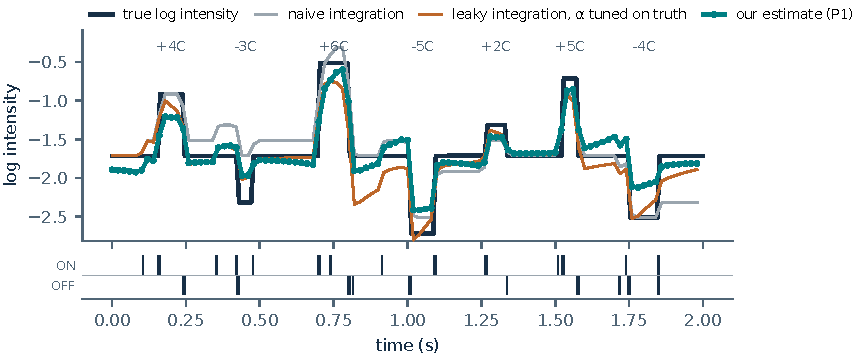
\includegraphics[width=\textwidth,height=5.3cm,keepaspectratio]{figures/synthetic_pixel/trace.pdf}\par
\vfill
% source: summary.json: 7 bars, 120 px/s, C = 0.2, shot 5 Hz, leak 0.1 Hz, sigma_C 0.03, 200 pixels, N = 100; median RMSE P1 0.191, leaky (oracle alpha 5) 0.216, naive 0.556; example pixel 55 events.
{\fontsize{6.5}{8}\selectfont\color{muted}Synthetic static camera: seven matte bars cross one pixel at 120\,px/s; labels give contrast in thresholds $C=0.2$. Sensor model with threshold mismatch, 5\,Hz shot noise, leak and refractory period. Median RMSE over 200 pixels: ours 0.19, leaky 0.22, naive 0.56.\par}
% source detail: synthetic experiment, November 2026; estimator configuration P1 (Gaussian 5 ms, sigmoid 0.03, sqrt), N = 100 over 2 s.
\src{Synthetic experiment, November 2026; Chapter~2 estimator, configuration P1; \dref{Theorem}{thm:frequency_response}.}
\talknote{Question: what does the estimate of one pixel look like over time? About 2 minutes.}{A static camera watches a gray background while seven bars of known reflectance pass one pixel. The true log intensity is the black staircase; the event raster underneath is what the pixel reports. Our estimate (teal) rises and falls with every bar and settles back on the background between bars. Naive integration (gray) keeps an offset after each pass from threshold mismatch and noise, and the offsets add up. Leaky integration (amber), with its decay rate tuned on the true signal, dips below the background after the dark bars. Over 200 pixels with independent sensor noise the median RMSE is 0.19 for ours, 0.22 for tuned leaky integration, and 0.56 for naive integration.}{This is the frequency response from the penalty slide in action: the baseline and slow drift are removed and passing edges are kept. The penalty constants are the MVSEC values, unchanged. Short bright bars come out about 0.3 below their peak, from the 5 ms kernel and the pull toward the background. The scene has exact ground truth at every instant, which the 30 Hz APS frames on MVSEC cannot give. The next slide repeats the comparison across noise levels.}
\end{frame}

\begin{frame}[label=pixelnoise]{The per-pixel estimate wins at every noise level}
% source: /scratch/dblauvel/ch2_synth_trace_20261120/passing/sweep.tsv (12 conditions: sigma_C 0.03, 0.06 x shot 1, 2, 5, 10, 20, 50 Hz, leak = shot/20); figure figures/synthetic_pixel/noise.pdf; exporter monocular_reconstruction/artifacts/defense_figures_20261120/export_synth.py.
\centering
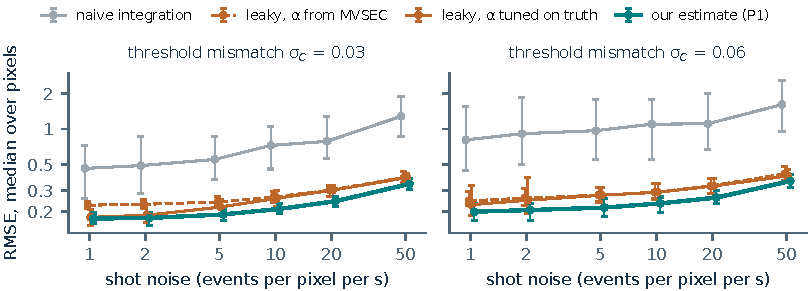
\includegraphics[width=\textwidth,height=5.6cm,keepaspectratio]{figures/synthetic_pixel/noise.pdf}\par
\vfill
% source: sweep.tsv: P1 lowest median RMSE in 12/12; vs oracle leaky 2% (1 Hz) and 5% (2 Hz) lower at sigma_C 0.03, 10-22% lower in the other 10; naive / P1 = 2.7-4.7.
{\fontsize{6.5}{8}\selectfont\color{muted}Same scene; 200 pixels per point, bars give the interquartile range. Leaky integration's decay rate is tuned on the true signal at each point (solid) or taken from MVSEC (dashed); our constants are the MVSEC values throughout.\par}
% source detail: synthetic experiment, November 2026; leaky alpha grid 0.5-100 s^-1 as in the MVSEC per-pixel comparison.
\src{Synthetic experiment, November 2026; Chapter~2 estimator, configuration P1.}
\talknote{Question: does the advantage hold as the sensor gets noisier? About 1 minute.}{Two levels of threshold mismatch, shot noise from 1 to 50 events per pixel per second. Our estimate has the lowest median error at all twelve points. Against leaky integration tuned on the true signal it is 2 and 5 percent lower at the two quietest settings and 10 to 22 percent lower at the other ten. Naive integration is 2.7 to 4.7 times higher.}{Doubling the threshold mismatch hurts naive integration most, because every pass leaves a residual. The leaky baseline here has an advantage it would not have in practice: its decay rate is chosen with the true signal. With the rate from MVSEC (dashed) it is 12 to 23 percent above ours.}
\end{frame}

% Opening views moved from the main talk: three-scene grayscale, MVSEC event views.
\begin{frame}[label=scenesgray]{Grayscale renderings of the three scenes}
% source: Ch. 2 subsubsec:datasets; ISS approx. 2 million events (f:iss), office approx. 2.5M events (subsec:validation_office), cup approx. 750,000 events (f:cup). Panels: figures/hook_p1/metadata.json (P1 configuration; ISS frame 31, office frame 29, cup frame 134); use the palette of the thesis cup false-color figure
\hookpanels[\reflectbox]{figures/hook_p1/iss_color.png}{figures/hook_p1/office_color.png}{figures/hook_p1/cup_color.png}
% source detail: Ch. 2, subsec:validation, f:iss, f:office, f:cup; datasets in subsubsec:datasets.
\src{\dref{Figure}{f:iss}, \dref{Figure}{f:office}, and \dref{Figure}{f:cup}; \dref{Section}{subsec:validation}. Data: Falcon Neuro~\cite{mcharg2022falcon}, office~\cite{gallego2017accurate}, cup~\cite{rebecq2021highspeed}.}
\talknote{Question: what do the three scenes look like without false color? About 30 seconds.}{The same reconstructed frames as the three-scene slide in the reconstruction section, in grayscale. Grayscale and false color are display choices for the same reconstructed relative brightness.}{ISS about 2 million events, office about 2.5 million, cup about 750 thousand; configuration P1, one per-pixel solve, no intensity frames.}
\end{frame}

\begin{frame}[label=mvsecevents3d]{Events record changes and the model supplies the level}
\begin{columns}[T]
\column{.30\textwidth}
\centering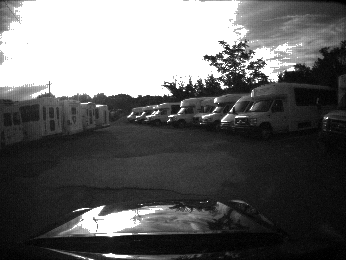
\includegraphics[width=\linewidth,height=2.6cm,keepaspectratio]{figures/mvsec_outdoor_day1/backup_p1/reference.png}\par\vspace{1mm}
{\small\textbf{Reference image}}
\column{.30\textwidth}
% source: figures/mvsec_outdoor_day1/backup_p1/metadata.json, events_3d (last 20 ms of the 50 ms event window; 13,221 events, 5,178 positive, 8,043 negative).
\centering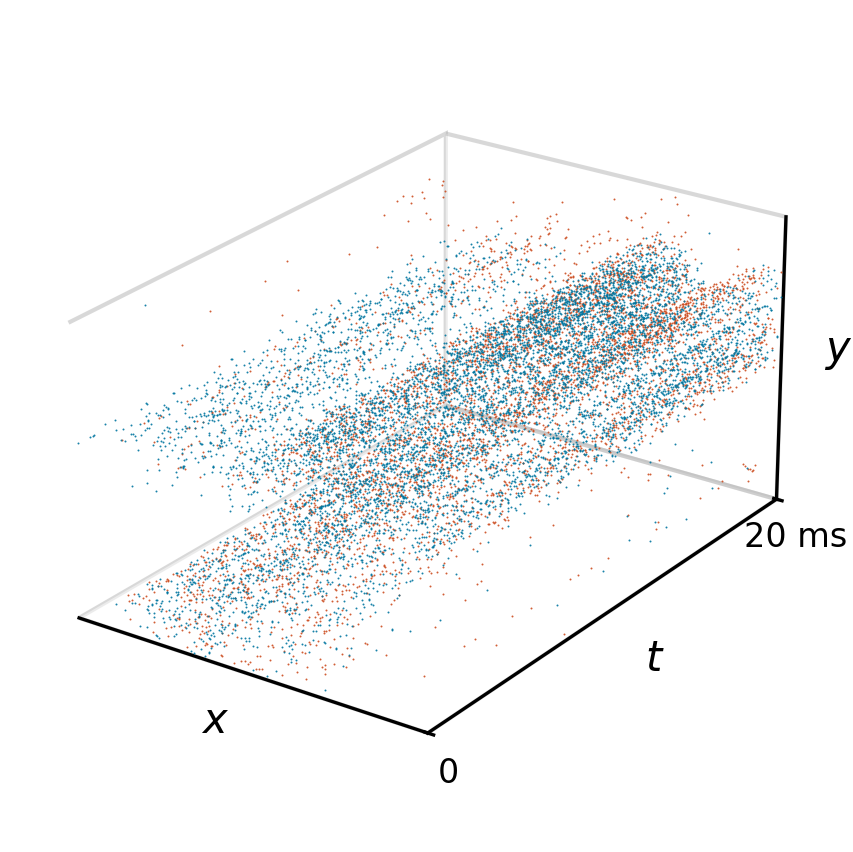
\includegraphics[width=\linewidth,height=2.6cm,keepaspectratio,trim=15 16 0 30,clip]{figures/mvsec_outdoor_day1/backup_p1/events_3d.png}\par\vspace{1mm}
{\small\textbf{Events in space and time}}\par
{\scriptsize $20$\,ms sample}\par
{\scriptsize\textcolor[RGB]{204,76,31}{Orange $+$}; \textcolor[RGB]{0,118,160}{blue $-$}.}
\column{.035\textwidth}
\vspace{1.1cm}\centering\textcolor{teal}{$\rightarrow$}
\column{.30\textwidth}
\centering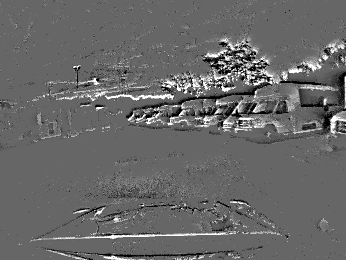
\includegraphics[width=\linewidth,height=2.6cm,keepaspectratio]{figures/mvsec_outdoor_day1/backup_p1/reconstruction.png}\par\vspace{1mm}
{\small\textbf{Our reconstruction}}
\end{columns}
\vspace{3mm}
{\large What do the observations determine, and what does the model supply?\par}
% source detail: Ch. 2 configuration P1 (Gaussian 5 ms, sigmoid), /scratch/dblauvel/ch2_recompute_20261103_p60/P1_gaussian_sigmoid_sqrt_0.03_n100/outdoor_day1, latent frame 29 of 100; exporter monocular_reconstruction/artifacts/defense_figures_20261108/export_backups.py.
% source: figures/mvsec_outdoor_day1/backup_p1/metadata.json, exact timing, raw-left geometry, normalization, and hashes.
\src{\dref{Chapter}{ch:monocular_reconstruction}, saved MVSEC~\cite{MVSEC2018} outdoor\_day1 reconstruction example.}
\talknote{Question: what does the raw event stream look like next to a reference image and a reconstruction? About 40 seconds.}{Left: a conventional reference image of the outdoor scene. Center: 20 ms of the event stream drawn as points in space and time, each dot one event at a pixel $(x,y)$ and a time $t$; orange is positive polarity, blue negative. Edges moving across the image sweep out the sheets of points. There are no frames, only a stream of change times. Right: our reconstruction.}{The 20 ms are the last part of the 50 ms window on the next slide: 13,221 events, 5,178 positive and 8,043 negative, raw left DAVIS geometry. Advance: the same events summed into one picture.}
\end{frame}

\begin{frame}[label=mvsecaccum]{Events record changes and the model supplies the level}
\begin{columns}[T]
\column{.30\textwidth}
\centering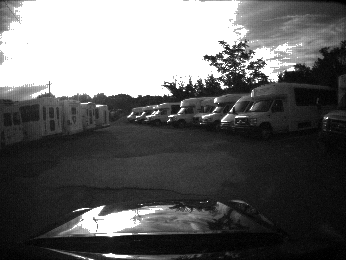
\includegraphics[width=\linewidth,height=2.6cm,keepaspectratio]{figures/mvsec_outdoor_day1/backup_p1/reference.png}\par\vspace{1mm}
{\small\textbf{Reference image}}
\column{.30\textwidth}
\centering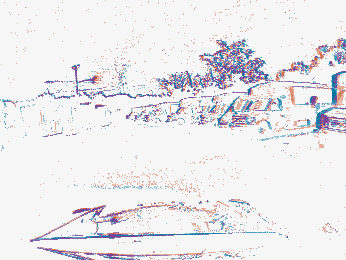
\includegraphics[width=\linewidth,height=2.6cm,keepaspectratio]{figures/mvsec_outdoor_day1/backup_p1/events_accumulation_orange_positive.png}\par\vspace{1mm}
{\small\textbf{Accumulated events}}\par
% source: figures/mvsec_outdoor_day1/backup_p1/metadata.json, event_panel (50 ms window ending at the frame time; color rule).
{\scriptsize $50$\,ms sample}\par
{\scriptsize\textcolor[RGB]{204,76,31}{Orange $+$}; \textcolor[RGB]{0,118,160}{blue $-$}; \textcolor[RGB]{119,70,151}{purple: both}.}
\column{.035\textwidth}
\vspace{1.1cm}\centering\textcolor{teal}{$\rightarrow$}
\column{.30\textwidth}
\centering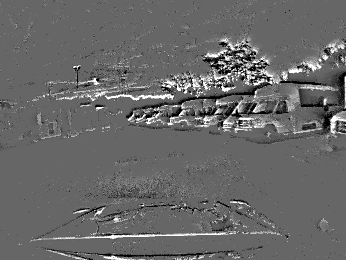
\includegraphics[width=\linewidth,height=2.6cm,keepaspectratio]{figures/mvsec_outdoor_day1/backup_p1/reconstruction.png}\par\vspace{1mm}
{\small\textbf{Our reconstruction}}
\end{columns}
\vspace{3mm}
{\large What do the observations determine, and what does the model supply?\par}
% source detail: Ch. 2 configuration P1 (Gaussian 5 ms, sigmoid), /scratch/dblauvel/ch2_recompute_20261103_p60/P1_gaussian_sigmoid_sqrt_0.03_n100/outdoor_day1, latent frame 29 of 100; exporter monocular_reconstruction/artifacts/defense_figures_20261108/export_backups.py.
% source: figures/mvsec_outdoor_day1/backup_p1/metadata.json, exact timing, raw-left geometry, normalization, and hashes.
\src{\dref{Chapter}{ch:monocular_reconstruction}, saved MVSEC~\cite{MVSEC2018} outdoor\_day1 reconstruction example.}
\talknote{Question: what do the events determine, and what does the model supply? About 60 seconds.}{Left is a conventional reference image of the outdoor scene. Center is a 50 ms sample of the event measurements used by the reconstruction: orange marks positive-only pixels, blue negative-only pixels, and purple pixels with both polarities. Right is our event-derived reconstruction with the selected Chapter 2 configuration, using a longer observation interval. The arrow represents events feeding the estimator; the reference supplies visual context. Events determine temporal changes, and the model selects a brightness baseline and how to balance observations with regularization.}{All panels use the raw left DAVIS geometry, $346\times260$ pixels. The 50 ms display interval ends at reconstruction time 1506118049.4719 s and contains 23,742 events. The reference is the nearest camera frame, 6.4 ms later. Reconstruction uses the full 500,000-event input spanning about 0.95 s; the center panel displays a subset of that input. Event color strength is logarithmic in count and saturates at four events per pixel. The reference is the saved 8-bit frame, unchanged; the reconstruction uses one affine mapping across its 100-frame sequence, background to mid-gray, then clips to $[0,1]$. This displays a latent event-derived state. The dissertation asks what observations determine, what penalties select, and what guarantees survive spatial or binocular coupling.}
\end{frame}

% Entries are generated from the dissertation .bbl; numbers are the dissertation numbers.
\begin{frame}[label=references]{References (1 of 3)}
\fontsize{6}{7.0}\selectfont
\begin{multicols}{2}
\thesisreferences{1}
\end{multicols}
\talknote{Reference list; navigation only.}{Numbers match the dissertation bibliography. Each bracketed number in the deck links here.}{Return to the slide under discussion with the PDF viewer's back command.}
\end{frame}

\begin{frame}{References (2 of 3)}
\fontsize{6}{7.0}\selectfont
\begin{multicols}{2}
\thesisreferences{2}
\end{multicols}
\talknote{Reference list; navigation only.}{Numbers match the dissertation bibliography. Each bracketed number in the deck links here.}{Return to the slide under discussion with the PDF viewer's back command.}
\end{frame}

\begin{frame}{References (3 of 3)}
\fontsize{6}{7.0}\selectfont
\begin{multicols}{2}
\thesisreferences{3}
\end{multicols}
\talknote{Reference list; navigation only.}{Numbers match the dissertation bibliography. Each bracketed number in the deck links here.}{Return to the slide under discussion with the PDF viewer's back command.}
\end{frame}
